%%%%%%%%%%%%%%%%%%%%%%%%%%%%%%%%%%%%%%%%%%%%%%%%%%%%%%%%%%%%%%%%%%%%%%
% amspaper.tex --  LaTeX-based template for submissions to American 
% Meteorological Society journals
%
% Template developed by Amy Hendrickson, 2013, TeXnology Inc., 
% amyh@texnology.com, http://www.texnology.com
% following earlier work by Brian Papa, American Meteorological Society
%
% Email questions to latex@ametsoc.org.
%
%%%%%%%%%%%%%%%%%%%%%%%%%%%%%%%%%%%%%%%%%%%%%%%%%%%%%%%%%%%%%%%%%%%%%
% PREAMBLE
%%%%%%%%%%%%%%%%%%%%%%%%%%%%%%%%%%%%%%%%%%%%%%%%%%%%%%%%%%%%%%%%%%%%%

%% Start with one of the following:
% DOUBLE-SPACED VERSION FOR SUBMISSION TO THE AMS
\documentclass{ametsoc}

% TWO-COLUMN JOURNAL PAGE LAYOUT---FOR AUTHOR USE ONLY
% \documentclass[twocol]{ametsoc}

%%%%%%%%%%%%%%%%%%%%%%%%%%%%%%%%
%%% To be entered only if twocol option is used

\journal{jcli}

\usepackage{color}

%  Please choose a journal abbreviation to use above from the following list:
% 
%   jamc     (Journal of Applied Meteorology and Climatology)
%   jtech     (Journal of Atmospheric and Oceanic Technology)
%   jhm      (Journal of Hydrometeorology)
%   jpo     (Journal of Physical Oceanography)
%   jas      (Journal of Atmospheric Sciences)	
%   jcli      (Journal of Climate)
%   mwr      (Monthly Weather Review)
%   wcas      (Weather, Climate, and Society)
%   waf       (Weather and Forecasting)
%   bams (Bulletin of the American Meteorological Society)
%   ei    (Earth Interactions)

%%%%%%%%%%%%%%%%%%%%%%%%%%%%%%%%
%Citations should be of the form ``author year''  not ``author, year''
\bibpunct{(}{)}{;}{a}{}{,}

%%%%%%%%%%%%%%%%%%%%%%%%%%%%%%%%

%%% To be entered by author:

%% May use \\ to break lines in title:

\title{High-resolution regional climate model evaluation using variable-resolution CESM over California}


%%% Enter authors' names, as you see in this example:
%%% Use \correspondingauthor{} and \thanks{Current Affiliation:...}
%%% immediately following the appropriate author.
%%%
%%% Note that the \correspondingauthor{} command is NECESSARY.
%%% The \thanks{} commands are OPTIONAL.

    \authors{Xingying Huang, \correspondingauthor{Xingying Huang, 
     Department of Land, Air and Water Resources,
     University of California Davis, Davis, CA 95616.}
  Alan M. Rhoades and Paul A. Ullrich}

     \affiliation{Department of Land, Air and Water Resources, University of Califonia, Davis}

\email{xyhuang@ucdavis.edu}


    \extraauthor{Colin M. Zarzycki}
    \extraaffil{National Center for Atmospheric Research}


%%%%%%%%%%%%%%%%%%%%%%%%%%%%%%%%%%%%%%%%%%%%%%%%%%%%%%%%%%%%%%%%%%%%%
% ABSTRACT
%
% Enter your Abstract here

\abstract{Understanding the effect of climate change at regional scales remains a topic with intensive researches. Due to computational constraints, high horizontal resolutions required to reach regional scales have been largely out of reach for current global climate models. However, high resolution is needed to represent fine-scale processes and topographic forcing, which is a significant driver of local climate variability. Although regional climate models (RCMs) have been widely used at these scales, variable-resolution global climate models (VRGCMs) have arisen as an alternative for studying regional weather and climate. In this paper, the recently developed variable-resolution option within the Community Earth System Model (CESM) is assessed for long-term regional climate modeling. The mean climatology of temperature and precipitation, across California's diverse climate zones, is analyzed and contrasted with the Weather Research and Forcasting (WRF) model (as a traditional RCM), regional reanalysis, gridded observational datasets and a uniform high-resolution CESM with the finite volume (FV) dynamical core. The results show that variable-resolution CESM is competitive in representing regional climatology on both annual and seasonal time scales. This assessment adds value to the use of VRGCMs for projecting climate change over the coming century and improve our understanding of both past and future regional climate related to fine-scale processes. This assessment is also relevant for addressing the scale limitation of current RCMs or VRGCMs when next-generation model resolution increases to $\sim$10km and beyond.} 



\begin{document}


%% Necessary!
\maketitle


%%%%%%%%%%%%%%%%%%%%%%%%%%%%%%%%%%%%%%%%%%%%%%%%%%%%%%%%%%%%%%%%%%%%%
% MAIN BODY OF PAPER
%%%%%%%%%%%%%%%%%%%%%%%%%%%%%%%%%%%%%%%%%%%%%%%%%%%%%%%%%%%%%%%%%%%%%
%
\section{Introduction}

Global climate models (GCMs) have been widely used to simulate both past and future climate. Although GCMs have demonstrated the capability to successfully represent large-scale features of the climate system, they are usually employed at coarse resolutions ($\sim$1$^\circ$), largely due to computational limitations. Global climate reanalysis datasets, which assimilate climate observations using a global model, represent a best estimate of historical weather patterns, but still have relatively low resolutions no finer than 0.5$^\circ$ (\url{http://reanalyses.org/atmosphere/overview-current-reanalyses}). Consequently, regional climate is not well captured by either GCMs or global reanalysis datasets.  However, dynamical processes at unrepresented scales are significant drivers for regional and local climate variability, especially over complex terrain \citep{soares2012wrf}. In order to capture these fine-scale dynamical features, high horizontal resolution is needed to allow for a more accurate representation of fine-scale forcings, processes and interactions \citep{leung2003regional, rauscher2010resolution}. With these enhancements, the regional climate information is expected to be more usable for policy makers and local stakeholders in formulating climate adaptation and mitigation strategies.

In order to model regional climate at high spatial and temporal resolution over a limited area, downscaling methods have been developed. There are largely two approaches for downscaling including statistical downscaling and dynamical downscaling. Dynamical downscaling is popular and commonly employed using nested limited-area models (LAMs) or by applying a variable resolution GCM (VRGCM) to model regional scales \citep{laprise2008regional}. In this context, LAMs are typically referred as regional climate models (RCMs) when applied to climate scales. Forced by output of GCMs or reanalysis data, RCMs have been widely used, particularly to capture physically consistent regional and local circulations at the needed spatial and temporal scales \citep{leung2003regional, christensen2007regional, bukovsky2009precipitation, mearns2012north}. Recently, VRGCMs have been increasingly employed for modeling regional climate. This approach uses a global model that includes high-resolution over a specific region and coarse resolution over the remainder of the globe \citep{staniforth1978variable, fox1997finite}. And there are different strategies to achieve high-resolution over the area of interest such as stretched-grid models or grid refinement technique \citep{fox1997finite, ringler2008multiresolution, skamarock2012multiscale}. VRGCMs have been demonstrated to be effective for regional climate studies and applications at a reduced computational cost compared to uniform GCMs \citep{fox2001variable, fox2006variable, rauscher2013exploring, zarzycki2015effects}. Fox et al. (2000) found that the stretched-grid version of a GCM captured not only large-scale meteorological patterns as traditional GCMs did but also mesoscale features especially when considering orographic forcing \citep{fox2000uniform}.

%The first is statistical downscaling, which aims to estimate fine scale behavior via analysis of the statistical relationships between observed small-scale variables and larger (GCM) scale variables \citep{fowler2007linking}. This method is empirical and cannot be used if the observed relationships do not hold under a changing climate. Dynamical downscaling, which uses a numerical model to simulate higher spatial resolution conditions in greater detail. 

Compared with RCMs, a key advantage of VRGCMs is that they use a single, unified modeling framework, rather than a separate GCM and RCM. Thus, VRGCMs avoid potential inconsistency between the global and regional domains, and naturally support two-way interaction between these domains without the need for nudging \citep{warner1997tutorial, mcdonald2003transparent, laprise2008challenging, mesinger2013limited}. However, in order to obtain deeper insight into the performance of these two modeling approaches, it is necessary to compare them directly. For the purposes of this paper, we will focus on the recently developed variable-resolution Community Earth System Model (varres-CESM) using the grid refinement technique as our VRGCM of interest. Although CESM has been well-used for uniform resolution modeling, variable-resolution in the Community Atmosphere Model�s (CAM) Spectral Element (SE) dynamical core has only been recently developed. \cite{zarzycki2014using} applied this option in CAM-SE and showed that high-resolution simulation of topical cyclones represented significant improvements over the unrefined simulation. Zarzycki et al. also compared the large-scale features of  varres-CESM 0.25$^\circ$ and uniform CESM at one degree, and found that adding refined region over the globe did not affect the global circulation noticeably \citep{zarzycki2014multidecadal, zarzycki2015effects}.

However, varres-CESM has yet to be rigorously investigated for long-term regional climate simulation \citep{taylor2010compatible, zarzycki2014using}. And in this paper, it is the first time to investigate whether VRGCMs can show similar or even better ability in regional climate modeling compared with traditional method of RCMs. The goal of this paper is to evaluate the performance of varres-CESM against gridded observational data, reanalysis data and in comparison to a RCM. Also, outputs from a uniform high-resolution CESM simulation have also been utilized here \citep{wehner2014resolution}. Our variable-resolution simulations will focus on relatively high resolutions for climate assessment, namely 28km and 14km grid spacing, which are much more typical for dynamically downscaled studies. For comparison with the more widely used RCM method, the Weather Research and Forecasting (WRF) model will be applied at 27km and 9km grid spacing \citep{skamarock2005coauthors}. The study focuses on models' ability to represent current climate statistics, particularly those relative to climate extremes. We anticipate that this assessment will add value in modeling mean regional climatology and improve our understanding about the effects of multi-scale processes in regional climate regulation. Our goal is also to advance the understanding of better use of models in future climate predictions and climatic extremes studies regionally.

In this paper, we use California (CA) as our study area. With its complex topography, coastal influences, and wide latitudinal range, this makes CA an excellent test bed. Also, an understanding of local climate variability is incredibly important for policymakers and stakeholders in California due to its vast agricultural industry, wide demographics, and vulnerability to anthropogenically-induced climate change \citep{hayhoe2004emissions, cayan2008overview}. RCM simulations over California have also been conducted in previous studies and showed the need of high resolution to better study regional climate and extreme events, especially over complex topography with large climate gradients \citep{leung2004mid, kanamitsu2007fifty, caldwell2009evaluation, pan2011influences, pierce2013probabilistic}. \cite{caldwell2009evaluation}, in particular, presented results from WRF (Weather Research and Forecasting) at 12km spatial resolution showing both the overall consistency and some biases (e.g. overestimation of precipitation) between simulations and observations.

This paper is organized as follows. Section 2 describes the model setup, verification data and evaluation methods. In section 3, results are demonstrated focusing on 2 m temperature (Ts) and precipitation (Pr). Key results are summarized along with further discussion in section 4.

%In almost all RCM studies, model precipitation was found to be overpredicted over the mountains of the west coast (a point discussed further in Section 3.1). Temperature biases seem to be more model dependent. Based on an intercomparison of 4 different RCM+GCM combinations, Duffy et al. (2006) also investigates model variances and precipitation- temperature correlation. 

%They should present the importance of studying California's climate at the beginning, which would make their objective more understandable. ???

%Among these studies, Kanamitsu et al. (2007) dynamically downscaled reanalysis data to 10-km resolution over CA showing the ability to study various regional climate phenomena within different time scales \citep{kanamitsu2007fifty}.

%paper: Exploring a Multi-resolution Approach Using AMIP Simulations_2015

\section{Models and Methodology}

\subsection{Simulation design} 

All simulations use the AMIP (Atmospheric Model Intercomparison Project) protocols \citep{Gates1992}. AMIP simulations attempt to recreate a climatology similar to that observed over the past few decades, with prescribed sea-surface temperatures (SSTs) and ice concentrations. 

\subsubsection{varres-CESM}

CESM is a state-of-the-art Earth modeling framework developed by the National Center for Atmospheric Research (NCAR), consisting of atmospheric, oceanic, land and sea ice components and has been heavily used for understanding the effects of global climate change \citep{neale2010description, hurrell2013community}. Different component models are connected by a couple component. In this way, the interfacial states and fluxes between the various component models are communicated and the fluxed quantities are conserved. Since we follow AMIP protocols in this study, communication is mainly occurred between atmospheric and land model. Ocean model and sean ice component are disabled. Here, CAM version 5 (CAM5) \citep{CAM5Tech} and the Community Land Model (CLM) version 4 \citep{CLM40Tech} are used. As mentioned earlier, SE was used as the dynamical core in CAM along with the variable-resolution grid support. The FAMIPC5 (F$\_$AMIP$\_$CAM5) compset was chosen for the simulations as it is the standard protocol for AMIP and is less computationally demanding.

For our study, the variable-resolution cubed-sphere grids are generated for use in CAM and CLM with the open-source software package SQuadGen \citep{ullrich2014squadgen}. The grids used are depicted in Figure \ref{fig:varres-CESM_map}.  The maximum horizontal resolution on these grids are 0.25 degree ($\sim$ 28km) and 0.125 degree ($\sim$ 14km) respectively, with one degree resolution covering the rest of the globe. These resolutions have been selected because CAM-SE naturally supports a 2:1 aspect ratio, meaning there are two transition layers from 1 degree to 0.25 degree, and one additional transition from 0.25 degree to 0.125 degree. The meteorological patterns (e.g. wind, pressure and precipitation) showed natural and conserved results over the transition boundary as described in \citep{zarzycki2015effects}. The time period is from 1979-01-01 to 2005-12-31 (UTC), and year 1979 was discarded as spin up time for CLM4.0. We chose this time period to present the recent historical climate and try to achieve the best balance between reproducibility and computational feasibility, which is further discussed in the Methodology part.

Variable-resolution topography files have been produced by starting with the National Geophysical Data Center (NGDC) 2-min ($\sim$ 3.5 km) Gridded Global Relief Dataset (ETOPO2v2) topography dataset and applying the differential smoothing technique by adjusting the c parameter from Eq. (1) in \cite{zarzycki2015effects}. The grid-scale topography is showed in Figure \ref{fig:topo}. The higher resolution simulations provide a much finer representation of regional topography. This is important for understanding local climate since topography is an important driver for fine-scale dynamic processes, especially over complex terrain.

Land surface datasets, and plant functional types, were created at the standard 0.50 degree resolution. Initialized conditions are provided for both CAM and CLM. Greenhouse gas (GHG) concentrations are prescribed based on historical observations. SSTs and ice coverage are supplied by the one degree Hadley Centre Sea Ice and Sea Surface Temperature dataset (HadISST) \citep{hurrell2008new}. Tuning parameters are not modified from their default configuration.

%F_AMIP_CAM5 (FAMIPC5)  Description: AMIP run for CMIP5 protocol with cam5 
%How do fields near the refinement boundary look, as compared to uniform resolution? The 2 way interaction of WRF is not conserving, while the 1:2 refinement is conserving. This needs to be discussed and diagnostics near the boundary with respect to conservation done. In particular a comparison of point forecasts and climate averaging needs to be done, to investigate the deviation of the non conserving model and if the climate averaging takes this effect away.

%the time step for different resolutions

\subsubsection{Uniform CESM} 

Output from a globally uniform CESM run at 0.25$^\circ$ spatial resolution is utilized for comparison. It helps us to see if variable-resolution CESM, which is at much lower computation cost than uniform one, can show comparable performance in modeling mean climatology \citep{bacmeister2014exploratory}. This globally uniform simulation uses the CAM5-FV (finite volume) dynamical core and is described in additional detail in \cite{wehner2014resolution} and \cite{wehner2014effect}. {\color{red} need to add details about this and which parameters are different from the public version.}

%Note that the appendix of the latter paper lists parameters that are different from the public release.

\subsubsection{WRF} 

WRF has gained wide acceptance in studying regional climate over the past decade, showing its adequate capability in representation of fine-scale climate properties \citep{lo2008assessment, leung2009atmospheric, soares2012wrf}. In this study, the fully compressible non-hydrostatic WRF model in version 3.5.1 with the Advanced Research WRF (ARW) dynamical solver is used. ERA (ECMWF re-analysis)-Interim data at surface and pressure-level was used to provide initial and lateral conditions for the domains. The lateral conditions and SSTs were updated every 6 hours. ERA-Interim reanalysis ($\sim$80 km) has been widely used and validated for its reliability as forcing data \citep{dee2011era}. Two simulations are conducted with finest horizontal resolution of 27km and 9km respectively, over the same time period as varres-CESM. The $\sim$10 km resolution is actually finer than most previous studies for long-term climate. Also, the year 1979 is used as a spin-up period and is discarded for purposes of analysis. 

The simulation domains of WRF are depicted in Figure \ref{fig:wrf_domains}. For the WRF 27km simulation, one domain is used. For the WRF 9km simulation, two nested domains are used with the outer domain at 27km (same as the WRF 27km) and inner domain at 9km horizontal grid resolution, satisfying the natural WRF refinement ratio of 3:1. As a common way in WRF, two-way nesting is enabled by feeding back information from the fine grid onto the coarse grid, thus the nested region's process of the coarse domain is replaced by the fine grid result \citep{skamarock2008time}. Both grids are centered on CA and have respectively, 120$\times$110 and 151$\times$172 grid points. Around the boundaries, 10 grid points are used as lateral relaxation zones. In order to reduce the drift between forcing data and RCM, grid nudging \citep{stauffer1990use} was applied to the outer domain every 6 hours at all levels except the planetary boundary layer (PBL) as suggested by \cite{lo2008assessment}. This setup uses 41 vertical levels with model top pressure at 50 hPa. The topography data used in 27km and 9km are interpolated from USGS (U.S. Geological Survey) elevation data with 10m and 2m resolution respectively. The grid-scale topography is contrasted in Figure \ref{fig:topo}. Some differences are also apparent between the 28km varres-CESM and 27km WRF model, particularly over the Central Valley, and indicative of a different methodology for preparation of the topography dataset.

%using all the meteorological and static data from nested domains as input.

Additionally, we used the following physics parameterizations: WSM (WRF Single-Moment) 6-class graupel microphysics scheme \citep{hong2006wrf}, Kain-Fritsch cumulus scheme \citep{kain2004kain}, CAM shortwave and longwave radiation schemes \citep{collins2004description}. These settings are supported by the one-year test running result with different options of cumulus scheme and radiation schemes. For the boundary layer, the Yonsei University scheme (YSU) \citep{hong2006new} and the Noah Land Surface Model \citep{chen2001coupling} were used. Both were chosen as they are common for climate applications that balance long-term reliability and computational cost.

%\subsection{Topography} 

\subsection{Datasets}

For validation purpose, available reanalysis and gridded observational datasets of the highest quality are employed (see Table \ref{tab:Datasets}). Although gridded observational datasets are generally based on measurements of weather stations, they are based on different network of stations. And these datasets are scaled and gridded using varied interpolation techniques, elevation models and processing algorithms. In this way, using multiple reference datasets rather than one is important to account for the uncertainties, when assessing the performance of the WRF and CESM simulations in terms of both mean behavior and variability. Moreover, in this study, our purpose of using these products is to serve as realistic proxies to allow for a comparison of the model results. We acknowledge that reanalysis products are particularly sensitive to model choice and choice of assimilated observations and so cannot be treated as truth. Detailed descriptions of these datasets are as follows.

%These data products incorporate station measurements or satellite information and other data. 

\paragraph{NARR:}  The North American Regional Reanalysis (NARR) provides dynamically downscaled data over North America at $\sim$ 32 km resolution and 3 hourly intervals from 1979 through present \citep{mesinger2006north}. It is National Centers for Environmental Prediction (NCEP)'s high resolution reanalysis product. All major climatological variables are present in NARR, making it an excellent candidate for assessment of regional climate. Nonetheless, some inaccuracies have been identified in NARR that must be accounted for, including deficiencies in precipitation fields away from the continental US \citep{bukovsky2007brief}.

%The NARR model uses the very high resolution NCEP Eta Model (32km/45 layer) together with the Regional Data Assimilation System (RDAS) which, significantly, assimilates precipitation along with other variables. (http://www.esrl.noaa.gov/psd/data/gridded/data.narr.html)

\paragraph{NCEP CPC:} This data set is CPC unified gauge-based analysis of daily precipitation provided by the National Oceanic and Atmospheric Administration (NOAA) Climate Prediction Center (CPC). It is a suite of unified precipitation products with consistent and improved quality by combining all information available at CPC and by taking advantage of the optimal interpolation (OI) objective analysis technique. The gauge analysis covers the Conterminous United States with a fine-resolution at 0.25$^\circ$ from 1948/01/01 to 2006/12/3.

%CPC: National Oceanic and Atmospheric Administration (NOAA) uses more stations than University of Washington (UW); http://www.esrl.noaa.gov/psd/data/gridded/data.unified.daily.conus.html

\paragraph{UW:} The UW daily gridded meteorological data is obtained from the Surface Water Modeling group at the University of Washington \citep{maurer2002long, hamlet2005production}. UW incorporated topographic corrections by forcing the long-term average precipitation to match that of the PRISM dataset. Temperature dataset is produced in a similar fashion as precipitation, but used a simple 6.1 K/km lapse rate for topographic effect. The dataset is at 0.125$^\circ$ horizontal resolution and provided from year 1949 to 2010.

\paragraph{PRISM:} The Parameter-elevation Regressions on Independent Slopes Model (PRISM) \citep{daly2008physiographically} supports a 4km gridded dataset obtained by taking wide range of point measurements and applying a weighted regression scheme that accounts for many factors affecting the local climatology. The datasets include total precipitation and minimum/maximum, (derived) mean temperatures and dewpoints, based on sophisticated quality control measures. Monthly climatological variables are available for 1895 through 2014 provided by the PRISM Climate Group. PRISM is U.S. Department of Agriculture (USDA)'s official climatological data. We will use this product as the main reference dataset for model assessment.

%PRISM is a set of monthly, yearly, and single-event gridded data products of mean temperature and precipitation, max/min temperatures, and dewpoints, primarily for the United States.The PRISM products use a weighted regression scheme to account for complex climate regimes associated with orography, rain shadows, temperature inversions, slope aspect, coastal proximity, and other factors.  PRISM Ts, on the other hand, is based on a larger network of station data and accounts for elevation and topographic effects in a much more sophisticated manner. 

\paragraph{Daymet:}  Daymet is an extremely high resolution (1 km) gridded dataset with daily outputs of total precipitation, humidity, and minimum/maximum temperature covering the years of 1980 through 2013 \citep{thornton1997generating, thornton1999improved, thornton2000simultaneous}. The dataset is produced using an algorithmic technique that ingests point station measurements in conjunction with a truncated Gaussian weighting filter.  Some adjustments are made to account for topography. Daymet is available through the Oak Ridge National Laboratory Distributed Active Archive Center (ORNL DAAC).

\subsection{Methodology}

Near surface (2 meter) temperature and precipitation have been analyzed over California, to assessing the models' performances in representing the mean climatology. Specifically, evaluation focuses on daily maximum, minimum and average 2m temperatures (Tmax, Tmin and Tavg), and daily precipitation (Pr). These variables are key for a baseline climate assessment, particularly for their relationship with water resources, agriculture and health. With the overall warm climate and large impact of heat waves over CA, we focus on the summer season covering June, July and August (JJA) in the aspect of temperature. Since the vast majority of precipitation in CA occurs in the winter season, together with the accumulation of snowpack, in this way, precipitation over December-January-February (DJF) is emphasized. 

%Those seasons also represent the most of the climate variability.

In order to adequately account for natural variability even at regional scale, simulations need to be run long enough \citep{solomon2007climate}. However, there is no particular timeframe for climatology studies. Average weather conditions over 30-year or so are typically used to track climate to make sure that the data is long enough to calculate an average that is not influenced by year-to-year variability \citep{dinse2009climate}. In this study, 26-year current-climate runtime is chosen to reasonably balance the reproducibility and computational availability. We have studied the variability of mean temperature and precipitation in both simulations and observations over 5, 10, 20 and 25 seasons or years, and the results showed that 20 or 25 years' simulation are long enough to adequately capture the regionally climate variability. 30 years or longer run time may sound better, but are not necessary for our case.

All the results showed in the following part are based on the time period from year 1980 to 2005. All the datasets have been investigated first to see if time trend exists over this 26 years period, and the least squares linear trend has been removed from original datasets if existing. It is found that for temperature, there do have statistically significant linear trend over some parts of CA under the two-tailed t-statistic significance level of 0.05. However, no significant trend has been detected for precipitation.

%https://www.ncl.ucar.edu/Document/Functions/Built-in/regCoef-1.shtml
%https://www.ncl.ucar.edu/Document/Functions/Built-in/cdft_p.shtml
%https://www.ncl.ucar.edu/Document/Functions/Built-in/dtrend_msg_n.shtmll; without remove the mean
%However, the linear trend is week with linear regression coefficient averaged around 0.5.

Further, in order to better assess the treatment of California's varied climate regions, the state has been divided into five regional zones, including: the Central Valley, Mountain Region, North Coast, South Coast, and Desert Region as showed in Figure \ref{fig:wrf_domains}. The division of these five zones are loosely based on the results of \cite{abatzoglou2009classification} and the building climates zones from California Energy Commission. For parts of the results analyses, simulations and datasets are masked to restrict climate variables to specific zones. We aim to examine the statistics of data averaged over geographic climate zones instead of just on grid-cell analysis. 

Statistical measurements have been used to quantify the performances of the models comparing with the reference datasets. These statistical variables include the Root-mean-square deviation (RMSD), mean absolute difference (MAD), mean relative difference (MRD) and correlation, and sample standard deviation. 

%RMSD is defined as the square root of (the sum of the square difference (models-reference) over each grid point of the study area/the numbers of the grid points)
%MAD is defined as the averaged absolute difference (models-reference) over all these grid points
%MRD is defined as the averaged relative difference ((models-reference)/reference) over all these grid points
%correlation is the uncentered pattern correlation, i.e. Pearson product-moment coefficient of linear correlation between models and reference datasets at corresponding locations
%sample standard deviation denoted by $s$, defined as the square root of (the sum of the square difference (x-xbar)/the numbers of the size), here the size are the number of years, the x is the value of each year for each grid point or averaged over each zone.

When calculating the difference at grid point, the reference datasets are remapped to the given model's output resolution. Datasets are remapped using a bilinear interpolation method, which has been verified to provide  satisfactory performance. Other remapping algorithms, such as patch-based have been tested and do not exhibit notable differences.

Student's t-test is used  when necessary to see if two sets of yearly or seasonly averaged data are significantly different from each other, and 0.05 is used as critical levels of significance. We need to point out that this is just a approximate test to further support our results analysis since the two populations being compared should follow a normal distribution.

%T-test 
%http://stattrek.com/regression/slope-test.aspx?Tutorial=AP
%The significance level for a given hypothesis test is a value for which a P-value less than or equal to is considered statistically significant. Typical values for are 0.1, 0.05, and 0.01. These values correspond to the probability of observing such an extreme value by chance.
%t test: https://www.ncl.ucar.edu/Document/Functions/Built-in/ttest.shtml

\section{Results}

\subsection{Temperature}

The mean JJA Tmax, Tmin and Tavg climatology over 26 years of simulations together with PRISM are shown in Figure \ref{fig:t2_JJA}. The statistical measurements over whole CA area are showed in Table \ref{tab:stat_JJA_t2}. We can see that all simulations have captured the spatial climate patterns showed by the PRISM, with high spatial correlations ($>$0.95), especially for Tmax and Tavg. For Tmax, comparing with reference datasets, varres-CESM showed a warmer climate generally with about 2 to 3$^\circ C$ difference. Uniform CESM is similar as varres-CESM, but with a larger RMSD value ($\sim$4$^\circ C$). However, WRF output displayed overall colder climate, especially the WRF 9km, with about 2 to 3$^\circ C$ difference. Tmax over Central Valley has been overestimated by all the simulations and the possible reason has been discussed at the end of this part.

For Tmin, varres-CESM still showed a warm effect ($\sim$3 to 4$^\circ C$), with a particularly egregious overestimation over Nevada. WRF also had overall warm effect but displayed better performance than varres-CESM with smaller differences ($\sim$2 to 3$^\circ C$), comparing with reference datasets. However, the pattern of Tmin presented in Figure \ref{fig:t2_JJA} in both WRF simulations suggests a cooler interior to the Central Valley and warmer perimeter, which is not supported by observations. Overestimation of Tmin and Tmax by varres-CESM leads a similar overestimation for Tavg, so does uniform CESM. And underestimation of Tmax by WRF, causes a underestimation for Tavg, but still statistically more close to reference datasets than CESMs. The sample standard deviations of the JJA Tmax, Tmin and Tavg by models and PRISM are showed in Figure \ref{fig:t2_JJA_std}. It can be seen that the variability has little changes across difference sub-zones, and the values are around 0.5 to 1.5 $^\circ C$ for all the datasets, except some higher values ($\sim$2$^\circ C$) over mountains regions in WRF 9km.

%the t test of the JJA Tmax, Tmin, Tavg for cesm 0.25d and cesm 0.125d showed they have about half region is significantly the same at the level 0.05.
% (although difference are much smaller when focusing exclusively on California)

There are some minor uncertainties, as we already discussed, showed when comparing with different reference datasets. We have made the Student's t-test to see if the JJA Tmax, Tmin and Tavg from PRISM, UW and Daymet are statistically different from each other. And the results showed that they are the same at the significance level of 0.05 over most regions of our study area, except coastal regions. These observations are still of the highest quality available and the uncertainty is relatively small compared with difference from the simulations, thus are unlikely impacting the evaluation results.

Overall, varres-CESM 0.125 degree performed best in simulating long-term Tmax, and WRF is better at modeling Tmin than varres-CESM. When comparing against NARR (not showed), the overestimation of Tmin are largely reduced for varres-CESM. This suggests that the source of the temperature bias in varres-CESM and NARR may be related. Additionally, there are a positive 2 K SST bias near the California coastline between varres-CESM and WRF runs. This may also cause overestimation of temperatures. The sea breeze effect, associated with cooler temperatures near the San Francisco Bay, are apparent in all runs. It is especially encouraging that differences in the varres-CESM simulations, which only used prescribed SSTs, closely matched those of WRF, which were forced at the lateral domain boundaries with reanalysis data. 

%However, these observations are still of the highest quality available and the uncertainty is relatively small compared with difference from the simulations. 
%Varres-CESM overestimated all JJA temperatures (especially Tmin), whereas WRF underestimates Tmax and Tavg.

%The RMSD values between the models and reference datasets range from $\sim$2 to 4$^\circ C$. It can still be seen that varres-CESM is comparable to WRF and uniform CESM, without meaning that they are statistically the same. 

%The DJF climatology is discussed here primarily due to its impact on snowpack. For Tmax (Figure \ref{fig:t2max_DJF}), all simulations show a warm bias over the Central Valley (that is especially pronounced for WRF 27 km), but a cold bias over almost all other regions (particularly in the mountain region of the WRF 9km simulations). For Tmin (Figure \ref{fig:t2min_DJF}), the model simulations show a warm bias over most regions except the mountain region. These errors were evidently smaller when comparing to PRISM rather than UW. For Tavg (lower part of Figure \ref{fig:t2avg_JJA&DJF}), biases are quite smaller between models and PRISM dataset. Overall, the RMSDs are still roughly between 1 and 3 K, as noted in Table \ref{tab:stat_DJF_t2}, but were slightly reduced from summertime RMSDs. Simulations at coarser resolution seem to perform better overall, especially for varres-CESM 0.25$^\circ$ in Tmax, however, varres-CESM 0.25$^\circ$ shows largest error in modeling Tmin. For varres-CESM, biases were largely unaffected by moving to higher resolutions, with a slight underprediction of Tmax and pronounced overprediction of Tmin.  Moving to higher resolutions with WRF greatly increased biases in all cases.

The seasonal cycle of Tavg is shown in Figure \ref{fig:trd_t2avg_allzones} for simulations and reference data from PRISM and NARR. The models do show good consistency with reference data with no larger than 2$^\circ C$ difference, which mainly occurred in the coldest and hottest seasons. Compared with PRISM, Varres-CESM showed positive difference over the summer season in all sub-zones except coastal regions, and negative difference over winter season in all zones, indicating larger temperature range. The uniform CESM is similar to varres-CESM, with about 1$^\circ C$ larger difference. WRF has better performance in presenting the monthly trend than CESM with about 1$^\circ C$ underestimation over all seasons. No notable differences can be discerned when comparing models across resolutions.

The variability over each month is expressed by the sample standard deviation showed in Figure \ref{fig:trd_t2avg_allzones_std}. Generally, local variability of Tavg is under 3$^\circ C$, mostly within the range from 1 to 2$^\circ C$. Among the simulations, WRF 27km is most consistent with PRISM. WRF 9km is also close to PRISM, but has $\sim$1$^\circ C$ larger variability over January and February. Varres-CESM basically showed about 0.5$^\circ C$ more scattered values (either above or lower) comparing to reference datasets, and uniform CESM has about 0.5$^\circ C$ lower variability than PRISM.

%Due to the disorganized change of monthly variability, it is not easy to interpret this figure.

For the temperature climatology in California, we are most interested in the Tmax over summer season due to the impact of summer heat waves. We depict the frequency distribution of Tmax using all the JJA daily values over 26 years. The results of the simulations and reference datasets of Daymet and UW are showed in Figure \ref{fig:PDF_t2max_allzones_JJA}. Properties of the frequency distribution, including average, variability, skewness and Kurtosis are tabulated in Table \ref{tab:PDF_t2max_JJA}. Though with some deviations, similar distribution shapes with tails off to left are present for both models and observations. Contrasting with WRF, varres-CESMs are more close to reference datasets. WRF 9km tended to be colder. Models including varres-CESM and WRF 27km are more consistent with observations for higher values than the peak and less consistent at lower values. For representation of heat extremes, both varres-CESM and WRF 27km exhibit satisfactory performance over most regions except in Central Valley (CV). No obvious improvement is associated with higher resolution in varres-CESM.

In the Central Valley, models show a clear warm effect and associated long tail, with temperatures reaching near 50$^\circ C$. As discussed before, all models do overestimate Tmax over CV. In order to further assess the accuracy of the gridded observations, we examine the Tmax data directly from recorded weather station observations over the CV. The results validate that Tmax values above 45$^\circ C$ are rare (although station observations suggest these days may be slightly more frequent than suggested by UW and Daymet). The warm bias associated with the aforementioned extreme hot days in both varres-CESM and WRF is likely correlated with overly dry summertime soil moisture, as discussed in \cite{caldwell2009evaluation}. This could be caused by the lack of accurate land surface treatment in climate models. areas. Bonfils and Lobell (2007) found that irrigation in Central Valley has significantly decreased summertime maximum temperatures especially in heavily-irrigated areas \citep{bonfils2007empirical}. Other studies have also found the cooling effects of irrigation, such as \citep{kueppers2007irrigation}.

%(0.14�C to 0.25�C per decade)

\subsection{Precipitation}

California is known for the shortage of natural water resources with extreme drought over summer season. In this way, the winter season is particularly important for California as it accounts for 50 percent of the $\sim$22.5 inches that California receives for its total annual average precipitation amounts (\url{http://www.ncdc.noaa.gov/cag/}).

The long-term average climatologies of DJF and annual daily precipitation (Pr) over 26 years from simulations and reference datasets are displayed in Figure \ref{fig:pr_DJF_Anuual}. And the statistical measurements over whole CA area are showed in Table \ref{tab:stat_Pr}. As we can see, precipitation is distributed mostly along the North coast and Sierra Nevada mountains, and is relatively sparse in other regions. As temperature, simulations also captured the spatial patterns of the PRISM, with high correlation coefficients ($>$0.94). However, there do exist clear differences among simulations.

Varres-CESM overestimated precipitation, especially in the coarser resolution (28 km) simulation (about 40$\%$-50$\%$) along the western side of Sierra Nevada, resulting statistical difference over this area comparing with PRISM. Interestingly, varres-CESM 0.125$^\circ$ is statistically the same as PRISM. Uniform CESM has slightly better results than varres-CESM 0.25deg. There are notable differences between WRF 27km and WRF 9km. WRF 27km underestimates precipitation for about 30$\%$, whereas WRF 9km shows a large positive difference (about 60$\%$-80$\%$) along the North coast and the Sierra Nevada. However, considering the variability showed in the Figure \ref{fig:pr_DJF_Annual_std}, WRF 9km and WRF 27km are both significantly the same at the significance level of 0.05 as PRISM except over the mountain region. From the sample standard deviation of the precipitation displayed in Figure \ref{fig:pr_DJF_Annual_std}, we can see that the variability has similar patterns of the precipitation intensity distribution, and increases as the precipitation magnitude increases. Models seem to capture the variation of precipitation well, particularly looking at the varres-CESM 0.125deg and WRF 27 km, though variability is $\sim$50$\%$ higher for WRF9km.

IThe reference datasets again showed differences indicating uncertainty inherent in interpolating station data to a grid. We have also made the Student's t-test to test the if the mean precipitation climatology from PRISM, UW and Daymet are statistically different from each other. And it turned out that they are almost the same at the significance level of 0.05 over all the study area. Therefore, the uncertainties within them are negligible. Overall, varres-CESM 0.125$^\circ$ performs slightly better than CESM 0.25$^\circ$ and WRF 27km, as further exhibited by the RMSD values in Table \ref{tab:stat_Pr}. 

The annual cycle of precipitation averaged over each sub-zone over 26 years is presented in Figure \ref{fig:trd_pr_allzones}. It can be seen that simulations showed similar trend as reference datasets. The main deviation occurred during the rainy seasons, especially in winter. WRF 27km is dryer and WRF 9km is far wetter in all regions as discussed above. Varres-CESM tracks well with observed precipitation everywhere except in the Central Valley, where precipitation is overestimated at rainy seasons with about 70$\%$-80$\%$. Nonetheless, the strong seasonal dependence on precipitation is apparent with extremely dry conditions during summer months. A slight increase in summertime precipitation is apparent in the Desert region, indicating the North American monsoon. Overall, varres-CESM is more consistent with observations compared with WRF. However, we also observe that the peak month for precipitation tends to occur earlier in varres-CESM than in observations. It is not surprising that a seasonal time drift occurred with the varres-CESM simulations as it was not forced by a reanalysis dataset (unlike the WRF simulations).

The variability over each month is expressed by the sample standard deviation showed in Figure \ref{fig:trd_pr_allzones_std}. The variability has similar monthly trend as the annual cycle of precipitation, with overall value from 0 to 4 mm$/$day, which generally shows higher inter-annual variability over locations of higher mean precipitation \ref{fig:trd_pr_allzones}. Comparing with observations, varres-CESM exhibited a slightly larger variability (basically no more than 1mm$/$day) in the rainy season, while WRF 27km has better representation with a little lower values. WRF 9km again showed larger variability (about $\sim$1mm$/$day more) during rainy seasons over most regions. Such higher variability within higher magnitude of precipitation has also been found in previous studies. Duffy et al. (2006) discussed the higher variability caused by higher spatial resolution used in RCM models, with more accurate representation of topography \citep{duffy2006simulations}. The main cause of the interannual variability of precipitation over CA is El Ni�o�Southern Oscillation (ENSO), which varies the amount of moisture flux transported to this region.

%The primary source of interannual variability in the study region is El Ni�o�Southern Oscillation (ENSO), which introduces variability primarily on times scales of 4 to 7 yr. This affects spatially averaged precipitation in the study region by varying the amount of moisture advected into the region.

The frequency distribution of DJF Pr has been constructed from rainy days in winter (Pr$>$=0.1mm/d) and depicted in Figure \ref{fig:PDF_pr_allzones_DJF}. Within our expectation, it can be seen that varres-CESM is more consistent with observations everywhere except in the CV. In this region WRF 27km appears to better capture high-intensity precipitation events, but performs more poorly on low-intensity events. The underestimation of rainfall frequency in WRF 27km appears consistent across regions. WRF 9km produces a significantly better treatment of low-intensity events, but greatly overestimates the frequency of high-intensity events. Notably, varres-CESM 0.25 degree and varres-CESM 0.125 degree do not show significant differences. For strong precipitation events, varres-CESM and WRF 27km show good performance over most regions except in those noted above, although these conclusions are also constrained by observational uncertainty.

The overestimation of precipitation for WRF at high resolution has also been found in previous studies. \cite{caldwell2009evaluation} showed that WRF at 12km largely overestimate the precipitation over the mountain division of CA. The deviation magnitude is less than what showed in this study due to different division area and perhaps different setting of physical schemes. In aforementioned Caldwell's paper, possible reasons have been discussed in detail, stating a variety of source including the model itself and the choice of physical parameterizations. A comprehensive analysis of the cause of these errors is beyond the scope of this paper. Further discussion can be found in former studies including the use of different microphysics schemes and resulting change of precipitation magnitude \citep{leung2003hydroclimate, jankov2005impact, gallus2006comparison, chin2010preliminary, caldwell2010california}.

Finally, a concise summary of model performance over CA is provided by the Taylor diagram (Figure \ref{fig:taylor_diagram}). This diagram includes the spatial centered correlation between the simulated and observed fields, the RMS variability of simulations normalized by that in the observations, and mean differences from reference data. It can be seen that the models correlate well with the PRISM reference dataset. Normalized standard deviation and bias are larger for precipitation, especially for WRF 9km. Overall, varres-CESM has demonstrated that it can competitively compare to WRF in capturing the regional climatology of California. ({\color{red}update the plot})

\section{Discussions and summary}

With the need of high resolution to better study regional climate and extreme events, this study got deep into the use of a variable-resolution GCM (i.e. varres-CESM) as an alternative way in dynamical regional climate modeling. The performance of varres-CESM has been investigated in simulating California climatology as regional climate studies. This relatively new technique has been evaluated against a traditional RCM (i.e. WRF) directly for the first time.
%SST higher resolution SST values

%To achieve this goal, uniform CESM is also included together with gridded reference datasets

Based on 26 years of high-resolution historical climate simulations, we analyzed the mean climatology of California and across its climate divisions from both temperature and precipitation, mainly based on the output of varres-CESM and WRF. Generally, when compared with gridded observational datasets, all simulations do a good job of capturing regional climatological patterns with high spatial correlations ($>$0.94). Uncertainty between reference datasets exists, but is relatively small and not statistically significant over most regions. We found that varres-CESM showed comparable performance as WRF in regional climate study. Even compared with a uniform high-resolution GCM (CESM-FV), varres-CESM also performed competitively.
%In the meantime, a uniform CESM simulation is also included. High-quality gridded datasets are used as reference datasets. 

Deviations from reference datasets do exist in these simulations, but they have different features. During summer, varres-CESM model possessed about 2 to 3$^\circ C$ warmer climate, especially in the Central Valley. WRF exhibited a colder ($\sim$2$^\circ C$) Tmax over most regions except the Central Valley, but a little warmer in Tmin. Overall, varres-CESM showed better ability in reproducing mean climatology of Tmax, but WRF was better at modeling Tmin and Tavg. The variability of JJA mean temperature is basically within the range of 0.5 to 1.5$^\circ C$. WRF presents the annual cycle of Tavg better than CESM with about 1$^\circ C$ underestimation. CESMs showed about 2$^\circ C$ overestimation of Tavg over the summer season and similar magnitude of underestimation over winter season, indicating larger temperature range over most regions.

For representation of heat extremes, both varres-CESM and WRF 27km exhibit close frequency to observations over all study area except in Central Valley (CV). This is likely caused by the lack of irrigation cooling effect over this region since irrigation is rarely considered in long-term climate modeling. In future work, we will add irrigation effect in varres-CESM to figure out the role irrigation played in regulating Tmax, and the overestimation and longer upbounded tail of frequency distribution for Tmax,

As for precipitation representation, varres-CESM overestimates winter or annual precipitation (about 40$\%$-50$\%$) especially along the western side of Sierra Nevada, and finer resolution simulation produces a slight reduction (10$\%$) likely due to improved treatment of orographic effects. WRF 27km underestimates precipitation (about 30$\%$) along the North coast and Sierra Nevada mountains, where almost all the precipitation comes from, whereas WRF 9km shows a large overestimation (about 70$\%$$-$80$\%$). Variability of precipitation ranges from 0 to 6 mm$/$day, with generally higher inter-annual variability over locations of higher mean precipitation. For strong precipitation events probalibity, varres-CESM and WRF 27km show satisfactory modeling ability over most regions (except at the Central Valley for varres-CESM), although the reference datasets also show some uncertainties.

%with main deviation occurred during the rainy seasons. Varres-CESM also exhibited a slightly larger variability than WRF 27km.  
%The main precipitation modeling deviations occurred during rainy seasons, especially in winter. 

Higher resolution (0.125$^\circ$) simulation of varres-CESM do show better results in capturing summer Tmax, precipitation and their variablility, than the coarser resolution run. However, the improvements are not statistically significant. For WRF, when resolution increased, the model produces obviously overestimated precipitation as previous studies have also found when using RCMs for fine-scale simulations as aforementioned. The use convection scheme is perhaps not needed when grid spacing is near 10km. However, it turned out that almost all of the precipitation comes from resolved (large-scale) processes for all these models. In this way, model deviation is mainly related with resolved-scale processes and microphysics scheme plays a major role, which makes it necessary to develop more scale-aware parameterizations. 

%Since our grid spacing is approaching the 10 km bound beyond which subgrid-scale (commonly referred to as �convective�) parameterizations are perhaps not needed (e.g. Dudhia et al. 2003).

The importance and necessity of high resolution for regional climate studies has been widely stressed by previous studies. However, whether the current regional climate models can fulfill this demand when resolution is pushed to local scales is questionable. It is clear that further work is urgently needed to solve the scale limitation of current regional climate models at fine horizontal resolutions. The possible causes of the scale limitation may include a lack of accurate scare-aware physical parameterizations near or below 10 km horizontal resolution, the treatment of dynamics at fine scales, and the interactions among different components of RCMs or VR-GCMs (e.g., land-atmosphere interactions). 

%A model�s performance can depend on horizontal resolution for different reasons: a more accurate representation of fine scale forcings (e.g. topography and land use), the better representation of processes and interactions (e.g. the dynamical structure of weather systems or cloud complexes; the location of major circulation features), and the direct dependence of physical parameterizations on the model grid size and time step interval.

In summary, varres-CESM demonstrated competitive utility for studying high-resolution regional climatology when compared to a regional climate model (WRF) and a uniform high-resolution GCM (CESM-FV). Deviations, showed within these models, are not indicative of deep underlying problems with the model formulation, but one should be aware of these differences when using these models for assessing future climate change. This study suggests that variable-resolution GCMs are useful tools for assessing climate change over the coming century. As the need for assessments of regional climate change is increasing, alternative modeling strategies, including variable-resolution global climate models will be needed to improve our understanding of the effects of fine-scale processes representation in regional climate regulation.


%%%%%%%%%%%%%%%%%%%%%%%%%%%%%%%%%%%%%%%%%%%%%%%%%%%%%%%%%%%%%%%%%%%%%
% ACKNOWLEDGMENTS
%%%%%%%%%%%%%%%%%%%%%%%%%%%%%%%%%%%%%%%%%%%%%%%%%%%%%%%%%%%%%%%%%%%%%
\acknowledgments

The authors would like to thank Michael Wehner and Da\'ith\'i Stone for providing the uniform resolution CESM dataset. We would further like to thank Travis O'Brien for his many useful conversations on climate model assessment. We also want to thank Xuemeng Chen for her assistance in WRF running. This project is supported in part by the University of California, Davis and by the Department of Energy ``Multiscale Methods for Accurate, Efficient, and Scale-Aware Models of the Earth System'' program.

 \bibliographystyle{ametsoc2014}
 \bibliography{database2015}

%\section{Figures and tables}

% TABLES

%%%%%%%%%%%Table1%%%%%%%%%%%%%%%%%%%%%%%
\begin{table}
\caption{Reanalysis and statistically downscaled observational datasets used in this study.} \label{tab:Datasets}
\begin{center}
\begin{tabular}{lcccc}
\hline \textbf{Data source} & \textbf{Variables used} & \textbf{Spatial resolution} & \textbf{Temporal resolution} \\
\hline \textbf{NARR} & Pr, T$_{s}$ & 32km & daily, 3-hourly \\
\textbf{NCEP CPC} & Pr & 0.125$^\circ$ & daily \\
\textbf{UW} & Pr, T$_{min}$, T$_{max}$ & 0.125$^\circ$ & daily \\
\textbf{PRISM} & Pr, T$_{min}$, T$_{max}$, T$_{avg}$ & 4km & monthly \\
\textbf{Daymet} & Pr, T$_{min}$, T$_{max}$ & 1km & daily \\
\hline
\end{tabular}
\end{center}
\end{table}


%%%%%%%%%%%Table2%%%%%%%%%%%%%%%%%%%%%%%
\begin{table}
\begin{center}
\caption{RMSD, MAD and Correlation (Corr) for JJA temperature over California} \label{tab:stat_JJA_t2}
\begin{tabular}{lcccc}
\hline \textbf{RMSD} & \textbf{UW}  & \textbf{PRISM} & \textbf{Daymet} \\
\hline $    $ & T$_{max}$ $\     $  T$_{min}$ & T$_{max}$ $\     $  T$_{min}$ $\     $ T$_{avg}$& T$_{max}$ $\     $  T$_{min}$\\
\hline \textbf{varres-CESM 0.25d} & 2.322 $\ $ 3.745 & 2.924 $\ $ 3.121 $\ $ 2.604 & 2.810 $\ $ 3.934 \\
\textbf{varres-CESM 0.125d} & 1.900 $\ $ 3.631 & 2.447 $\ $ 2.944 $\ $ 2.184 & 2.475 $\ $ 3.701 \\
\textbf{WRF 27km} & 2.310 $\ $ 2.738 & 2.933 $\ $ 2.254 $\ $ 2.169 & 2.511 $\ $ 2.992 \\
\textbf{WRF 9km} & 3.319 $\ $ 2.937 & 3.492 $\ $ 1.837 $\ $ 1.769 & 3.203 $\ $ 2.942 \\
\textbf{uniform CESM 0.25d} & 3.885 $\ $ 4.088 & 4.265 $\ $ 3.614 $\ $ 3.536 & 4.315 $\ $ 4.274 \\
\hline
\end{tabular}

\begin{tabular}{lcccc}
\hline \textbf{MAD} & \textbf{UW}  & \textbf{PRISM} & \textbf{Daymet} \\
\hline $    $ & T$_{max}$ $\     $  T$_{min}$ & T$_{max}$ $\     $  T$_{min}$ $\     $ T$_{avg}$& T$_{max}$ $\     $  T$_{min}$\\
\hline \textbf{varres-CESM 0.25d} & 0.981 $\ $ 2.907 & 0.606 $\ $ 1.731 $\ $ 0.823 & 1.177 $\ $ 2.877 \\
\textbf{varres-CESM 0.125d} & 0.645 $\ $ 2.848 & 0.203 $\ $ 1.660 $\ $ 0.579 & 0.818 $\ $ 2.744 \\
\textbf{WRF 27km} & -0.577 $\ $ 0.819 & -0.952 $\ $ -0.357 $\ $ -0.771 & -0.386 $\ $ 0.789 \\
\textbf{WRF 9km} & -2.277 $\ $ 1.862 & -2.720 $\ $ 0.674 $\ $ -1.142 & -2.103 $\ $ 1.757 \\
\textbf{uniform CESM 0.25d} & 1.812 $\ $ 2.993 & 1.449 $\ $ 1.815 $\ $ 1.280 & 2.013 $\ $ 2.961 \\
\hline
\end{tabular}

\begin{tabular}{lcccc}
\hline \textbf{Corr} & \textbf{UW}  & \textbf{PRISM} & \textbf{Daymet} \\
\hline $    $ & T$_{max}$ $\     $  T$_{min}$ & T$_{max}$ $\     $  T$_{min}$ $\     $ T$_{avg}$& T$_{max}$ $\     $  T$_{min}$\\
\hline \textbf{varres-CESM 0.25d} & 0.998 $\ $ 0.982 & 0.996 $\ $ 0.986 $\ $ 0.994 & 0.997 $\ $ 0.979 \\
\textbf{varres-CESM 0.125d} & 0.998 $\ $ 0.985 & 0.997 $\ $ 0.988 $\ $ 0.996 & 0.997 $\ $ 0.983 \\
\textbf{WRF 27km} & 0.997 $\ $ 0.982 & 0.996 $\ $ 0.989 $\ $ 0.996 & 0.997 $\ $ 0.978 \\
\textbf{WRF 9km} & 0.996 $\ $ 0.985 & 0.997 $\ $ 0.993 $\ $ 0.998 & 0.996 $\ $ 0.984 \\
\textbf{uniform CESM 0.25d} & 0.994 $\ $ 0.980 & 0.992 $\ $ 0.981 $\ $ 0.991 & 0.993 $\ $ 0.977 \\
\hline
\end{tabular}
\end{center}
\end{table}

%%%%%%%Table3%%%%%%%%%%%%%%%%%%%%%%%%%%%%%%

\begin{table}
\begin{center}
\caption{The first four moments of the JJA Tmax frequency in each sub-zone.  Column titles refer to Average (Avg), Variance (Var), Skewness (Skew) and Kurtosis (Kurt).} \label{tab:PDF_t2max_JJA}
\begin{tabular}{lccccc}
\hline \textbf{} & \textbf{Central valley}  & \textbf{Mountain} & \textbf{North coast} & \textbf{South coast} &\textbf{Desert}\\
\hline & Avg $\ $\ $ Var$\ $\ $Skew$\ $\ $ Kurt$ & Avg $\ $\ $ Var$\ $\ $Skew$\ $\ $ Kurt$  & Avg $\ $\ $ Var$\ $\ $Skew$\ $\ $ Kurt$  & Avg $\ $\ $ Var$\ $\ $Skew$\ $\ $ Kurt$  & Avg $\ $\ $ Var$\ $\ $Skew$\ $\ $ Kurt$  \\
\hline \textbf{UW} &32.6$\ $	24.8	$\ $-0.8$\ $	0.9	&	26.7	$\ $33.2$\ $	-0.4	$\ $0.3	&	25.9	$\ $30.4	$\ $0.1$\ $	-0.5		&25.9$\ $	30.4	$\ $0.1$\ $	-0.5&		37.0	$\ $22.9$\ $	-0.6	$\ $0.7\\
\textbf{Daymet} & 32.7$\ $	23.5$\ $	-0.9$\ $	1.5	&	25.9	$\ $39.3$\ $	-0.5$\ $	0.5	&	26.5	$\ $30.1	$\ $-0.3$\ $	0.4	&	26.5	$\ $30.1	$\ $-0.3	$\ $0.4		& 37.0	$\ $24.3	$\ $-0.6$\ $	0.6\\
\hline\textbf{CESM 0.25d}& 34.1$\ $	26.2	$\ $-0.4$\ $	0.2	&	28.1	$\ $27.6$\ $	-0.4$\ $	0.3	&	26.4	$\ $37.4	$\ $0.1$\ $	-0.7		& 26.4$\ $	37.4	$\ $0.1$\ $	-0.7	&	37.6$\ $	19.0$\ $	-0.5	$\ $0.8\\
\textbf{CESM 0.125d}& 34.3	$\ $28.5$\ $	-0.5	$\ $0.4	&	27.2	$\ $30.0$\ $	-0.4$\ $	0.3	&	26.3	$\ $37.4$\ $	0.1$\ $	-0.6		& 26.3$\ $	37.4$\ $	0.1	$\ $-0.6		& 37.3	$\ $21.3$\ $	-0.5	$\ $0.4\\
\hline\textbf{WRF 27km} & 33.9	$\ $34.8	$\ $-0.5$\ $	0.2	&	24.9	$\ $34.8$\ $	-0.3	$\ $0.0	&	26.0	$\ $36.7	$\ $-0.1$\ $	-0.5		& 26.0$\ $	36.7	$\ $-0.1	$\ $-0.5		& 36.5$\ $	22.6$\ $	-0.6$\ $	0.5\\
\textbf{WRF 9km}&32.4		$\ $33.1	$\ $	-0.7	$\ $	0.6	&	22.4		$\ $38.5		$\ $-0.5		$\ $0.6	&	24.9	$\ $	32.6		$\ $0.0		$\ $-0.6	&	24.9	$\ $	32.6	$\ $	0.0		$\ $-0.6	&	34.4		$\ $24.4		$\ $-0.5		$\ $0.4\\
\hline
\end{tabular}
\end{center}
\begin{tabular}{p{6in}}
\textbf{Notes:} If skew $>0$ [skew $<0$], the distribution trails off to the right [left]. If kurtosis $> 0$ [$<0$], it is usually more sharply peaked [flatter] than the normal distribution (leptokurtic and platykurtic, respectively).
\end{tabular}
\end{table}

%%%%%%Table4%%%%%%%%%%%%%%%%%%%%%%%%%%%

\begin{table}
\begin{center}
\caption{RMSD, MAD, MRD, Correlation (Corr) for precipitation over California} \label{tab:stat_Pr}
\begin{tabular}{lcccc}
\hline \textbf{Annual} & \textbf{CPC}  & \textbf{UW} & \textbf{PRISM} & \textbf{DAYMET} \\
\hline $    $ & RMSD $\ $ MAD $\ $ MRD $\ $ Corr & RMSD $\ $ MAD $\ $ MRD $\ $ Corr & RMSD $\ $ MAD $\ $ MRD $\ $ Corr & RMSD $\ $ MAD $\ $ MRD $\ $ Corr \\
\hline \textbf{varres-CESM 0.25d} & 0.607 $\ $ 0.394 $\ $ 0.413 $\ $ 0.981 & 0.616 $\ $ 0.292 $\ $ 0.434 $\ $ 0.968 & 0.727 $\ $ 0.203 $\ $ 0.429 $\ $ 0.952 & 0.567 $\ $ 0.191 $\ $ 0.375 $\ $ 0.972 \\
\textbf{varres-CESM 0.125d} & 0.469 $\ $ 0.207 $\ $ 0.321 $\ $ 0.980 & 0.526 $\ $ 0.115 $\ $ 0.339 $\ $ 0.970 & 0.624 $\ $ 0.045 $\ $ 0.328 $\ $ 0.961 & 0.504 $\ $ 0.027 $\ $ 0.310 $\ $ 0.973 \\
\textbf{WRF 27km} & 0.419 $\ $ -0.205 $\ $ 0.269 $\ $ 0.977 & 0.580 $\ $ -0.308 $\ $ 0.274 $\ $ 0.971 & 0.765 $\ $ -0.396 $\ $ 0.296 $\ $ 0.965 & 0.647 $\ $ -0.409 $\ $ 0.312 $\ $ 0.970 \\
\textbf{WRF 9km} & 2.226 $\ $ 1.485 $\ $ 0.950 $\ $ 0.957 & 2.052 $\ $ 1.393 $\ $ 0.864 $\ $ 0.964 & 1.889 $\ $ 1.322 $\ $ 0.815 $\ $ 0.970 & 2.005 $\ $ 1.306 $\ $ 0.773 $\ $ 0.961 \\
\textbf{uniform CESM 0.25d} & 0.555 $\ $ 0.134 $\ $ 0.277 $\ $ 0.969 & 0.600 $\ $ 0.031 $\ $ 0.302 $\ $ 0.961 & 0.700 $\ $ -0.057 $\ $ 0.290 $\ $ 0.953 & 0.600 $\ $ -0.069 $\ $ 0.284 $\ $ 0.962 \\
\hline
\end{tabular}

\begin{tabular}{lcccc}
\hline \textbf{DJF} & \textbf{CPC}  & \textbf{UW} & \textbf{PRISM} & \textbf{DAYMET} \\
\hline $    $ & RMSD $\ $ MAD $\ $ MRD $\ $ Corr & RMSD $\ $ MAD $\ $ MRD $\ $ Corr & RMSD $\ $ MAD $\ $ MRD $\ $ Corr & RMSD $\ $ MAD $\ $ MRD $\ $ Corr \\
\hline \textbf{varres-CESM 0.25d} & 1.486 $\ $ 0.986 $\ $ 0.532 $\ $ 0.972 & 1.445 $\ $ 0.673 $\ $ 0.531 $\ $ 0.959 & 1.654 $\ $ 0.577 $\ $ 0.547 $\ $ 0.943 & 1.346 $\ $ 0.514 $\ $ 0.435 $\ $ 0.964 \\
\textbf{varres-CESM 0.125d} & 1.194 $\ $ 0.638 $\ $ 0.396 $\ $ 0.976 & 1.234 $\ $ 0.346 $\ $ 0.398 $\ $ 0.965 & 1.395 $\ $ 0.287 $\ $ 0.400 $\ $ 0.955 & 1.170 $\ $ 0.212 $\ $ 0.337 $\ $ 0.969 \\
\textbf{WRF 27km} & 0.888 $\ $ -0.376 $\ $ 0.269 $\ $ 0.975 & 1.289 $\ $ -0.688 $\ $ 0.289 $\ $ 0.967 & 1.552 $\ $ -0.785 $\ $ 0.298 $\ $ 0.962 & 1.351 $\ $ -0.848 $\ $ 0.324 $\ $ 0.966 \\
\textbf{WRF 9km} & 4.264 $\ $ 2.607 $\ $ 0.742 $\ $ 0.950 & 3.835 $\ $ 2.315 $\ $ 0.616 $\ $ 0.955 & 3.570 $\ $ 2.256 $\ $ 0.604 $\ $ 0.964 & 3.804 $\ $ 2.183 $\ $ 0.554 $\ $ 0.955 \\
\textbf{uniform CESM 0.25d} & 1.392 $\ $ 0.377 $\ $ 0.300 $\ $ 0.960 & 1.431 $\ $ 0.064 $\ $ 0.316 $\ $ 0.951 & 1.544 $\ $ -0.033 $\ $ 0.314 $\ $ 0.946 & 1.406 $\ $ -0.095 $\ $ 0.288 $\ $ 0.953 \\
\hline
\end{tabular}
\end{center}
\end{table}

%\subsection{Figures}

\begin{figure}
\begin{center}
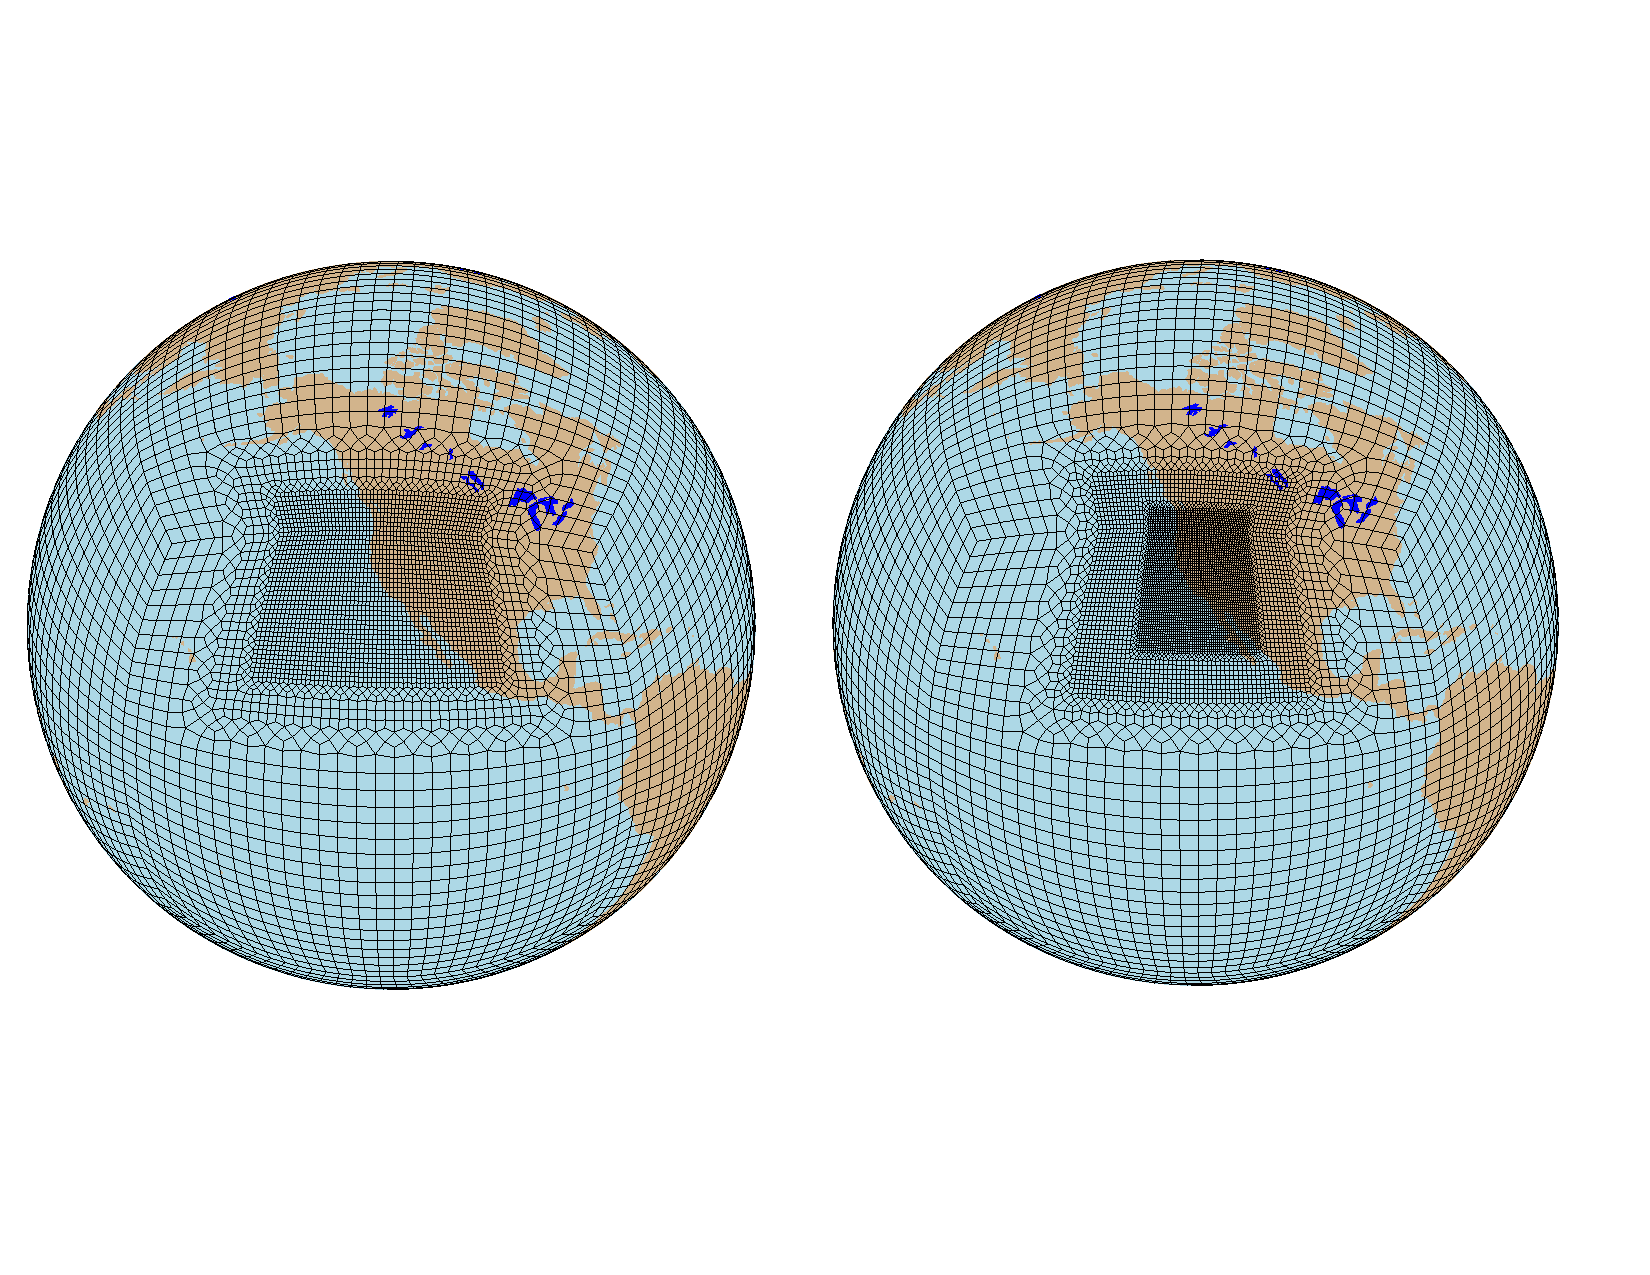
\includegraphics[width=6in]{varres-cesm_gridmesh.pdf}
\end{center}
\caption{Grid meshes for the two varres-CESM simulations.} \label{fig:varres-CESM_map}
\end{figure}

%Approximate regional resolution for the computational grids used in varres-CESM simulations.  The dashed lines and solid lines correspond to the outer boundary and inner boundary of the transition region.

\begin{figure}
\begin{center}
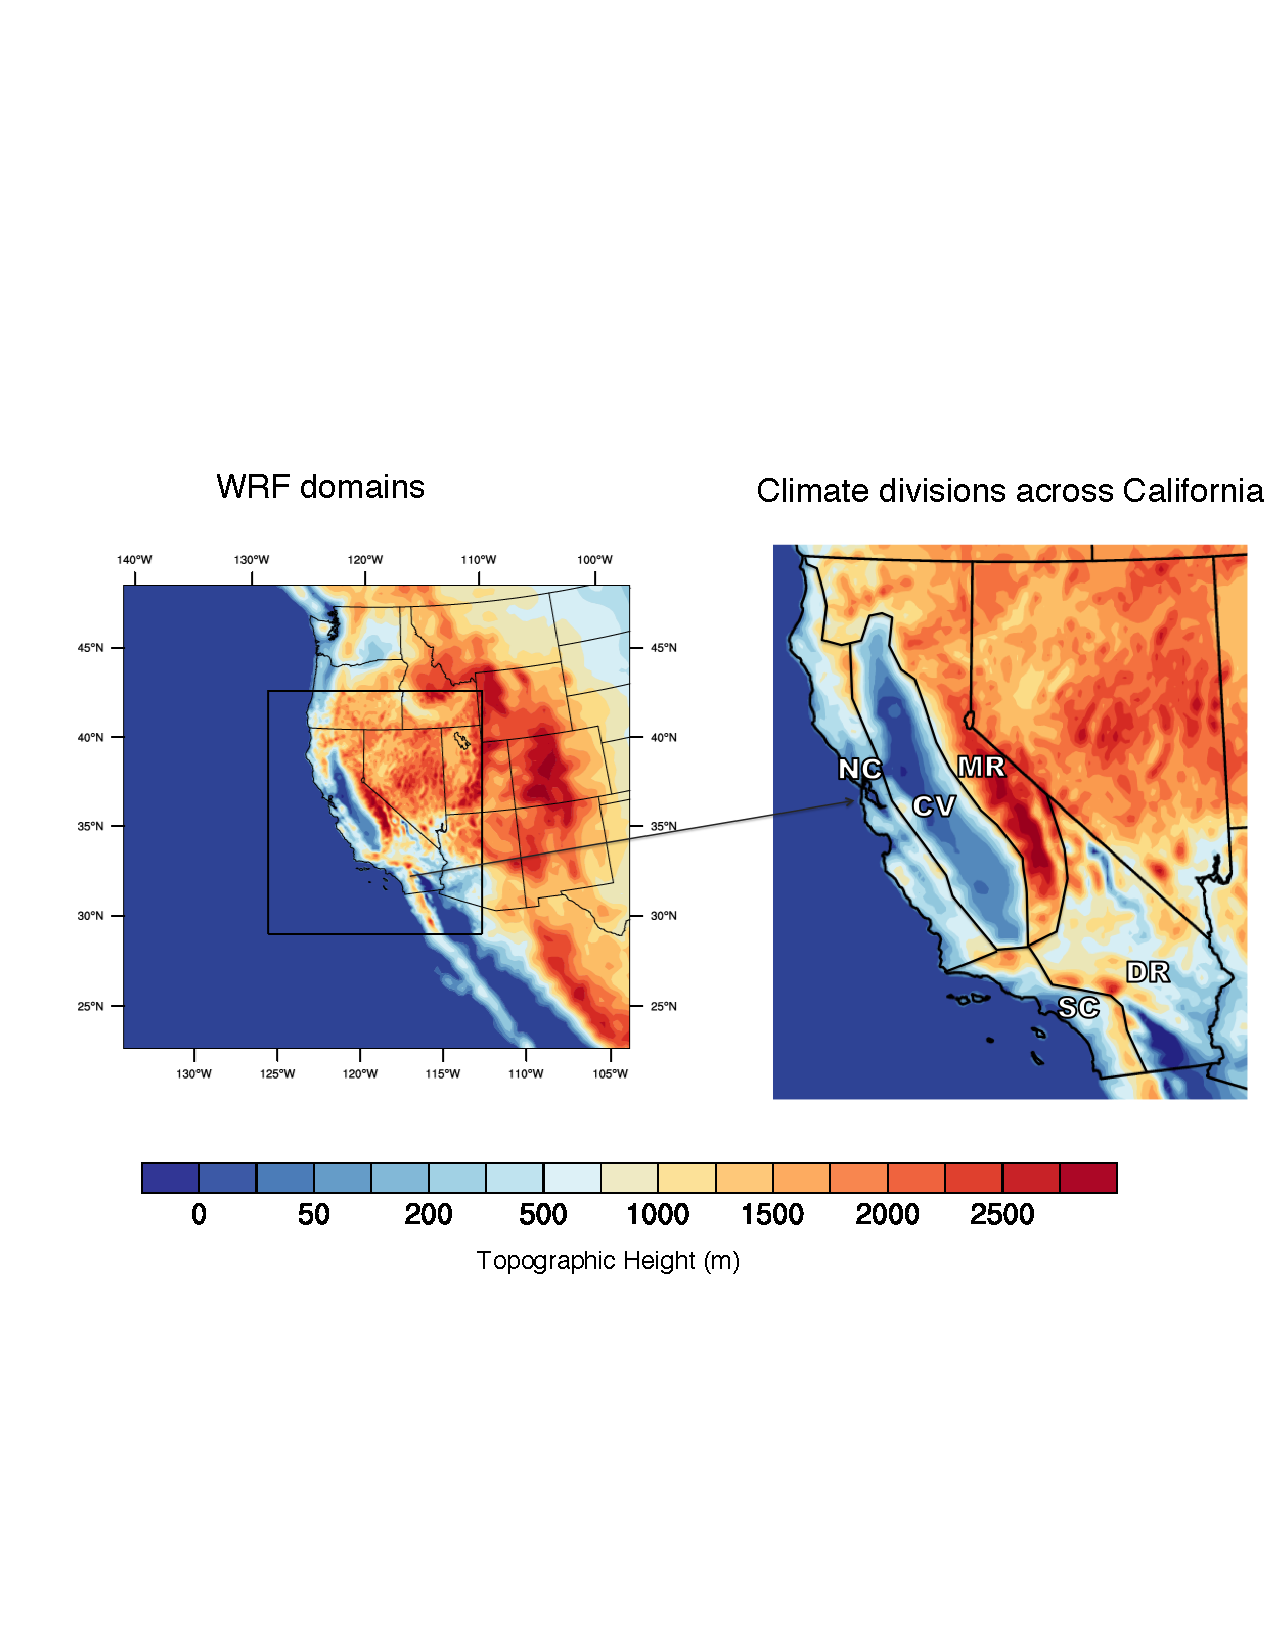
\includegraphics[width=6in]{wrf_domains.pdf}
\end{center}
\caption{Domains of WRF simulations (left) and five climate divisions in California (right) with topography in meters (m). } \label{fig:wrf_domains}
\end{figure}

\begin{figure}
\begin{center}
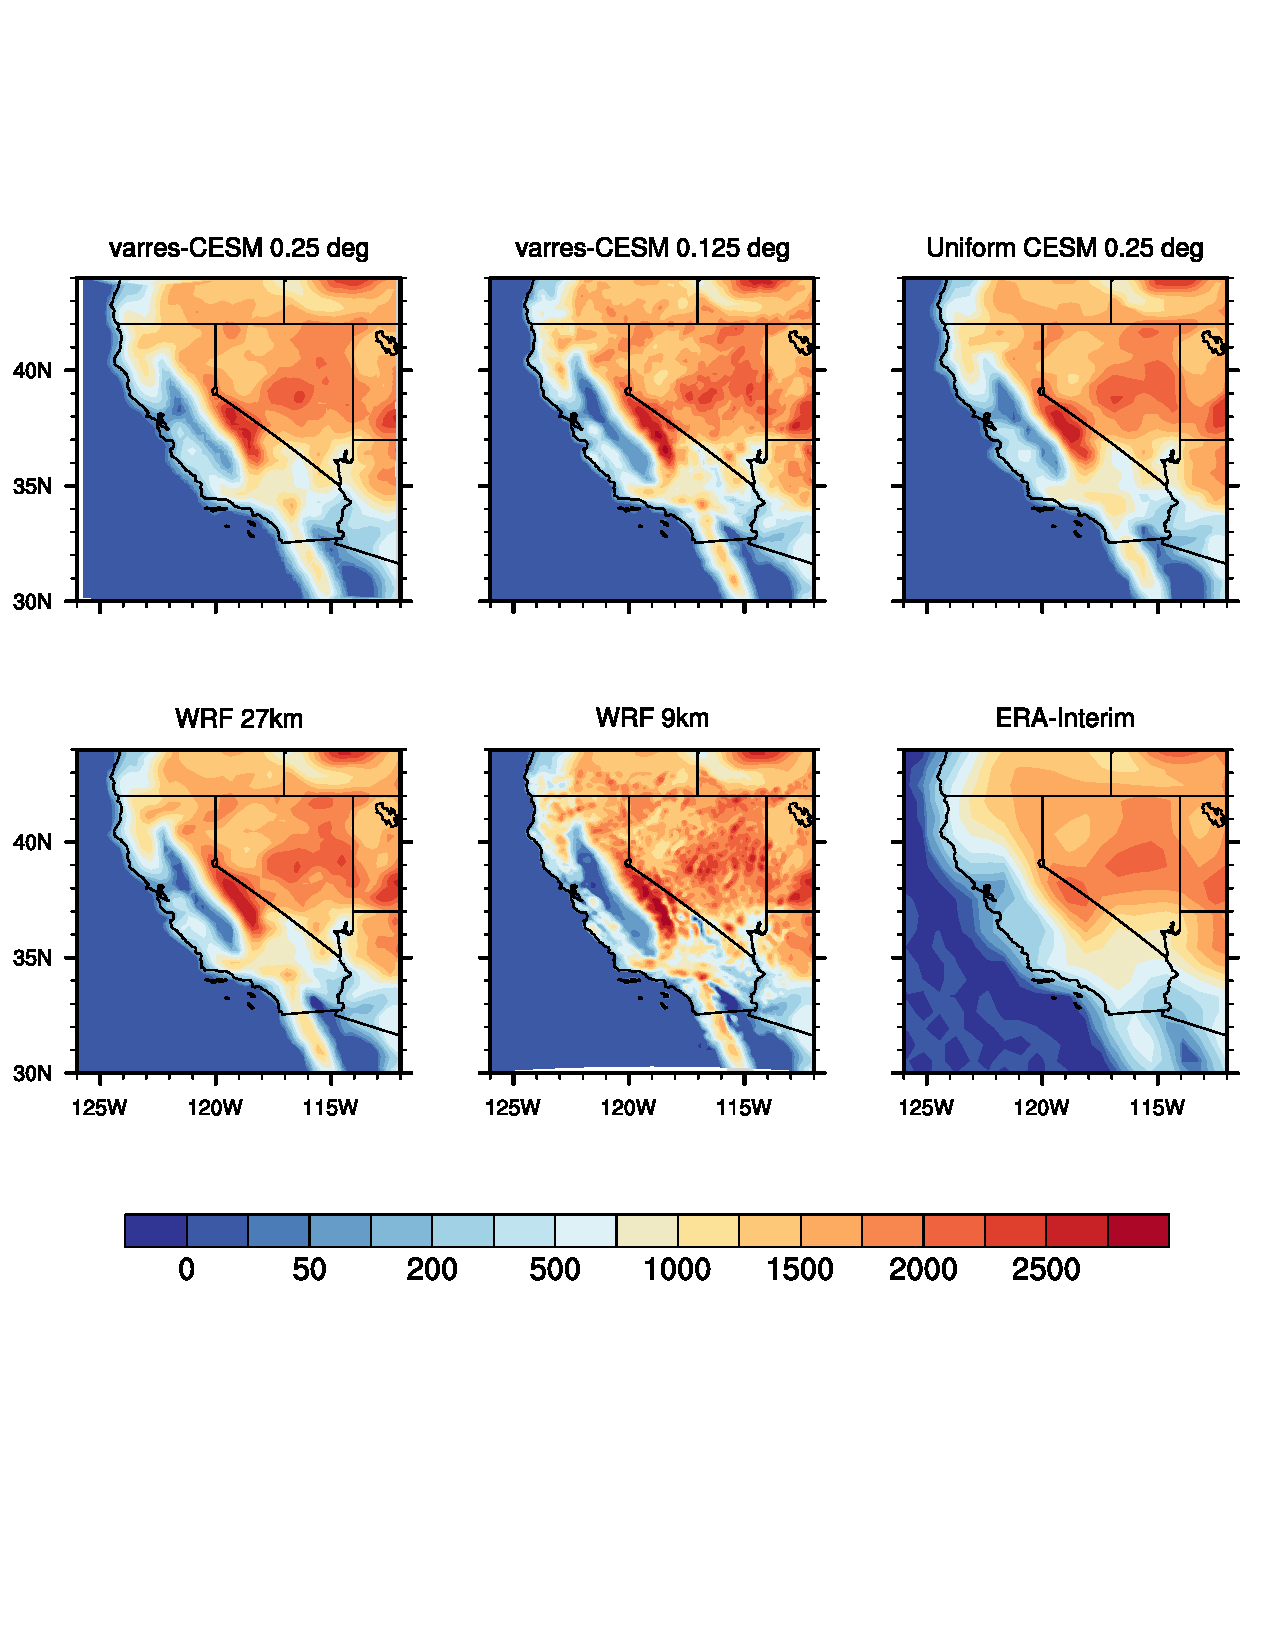
\includegraphics[width=6in]{topo.pdf}
\end{center}
\caption{Topography in meters (m) for (top left to bottom right) varres-CESM 0.25$^\circ$, varres-CESM 0.125$^\circ$, uniform CESM-FV 0.25$^\circ$, WRF 27km, WRF 9km and ERA-Interim ($\sim$80 km).} \label{fig:topo} 
\end{figure}

\begin{figure}
\begin{center}
\includegraphics[width=6in]{t2_JJA.pdf}
\end{center}
\caption{JJA average daily Tmax, Tmin and Tavg from models and reference datasets, and differences between them ($^\circ$C).} \label{fig:t2_JJA}
\end{figure}

\begin{figure}
\begin{center}
\includegraphics[width=6in]{t2_JJA_std.pdf}
\end{center}
\caption{sample standard deviation of JJA average daily Tmax, Tmin and Tavg from models and PRISM ($^\circ$C).} \label{fig:t2_JJA_std}
\end{figure}

\begin{figure}
\begin{center}
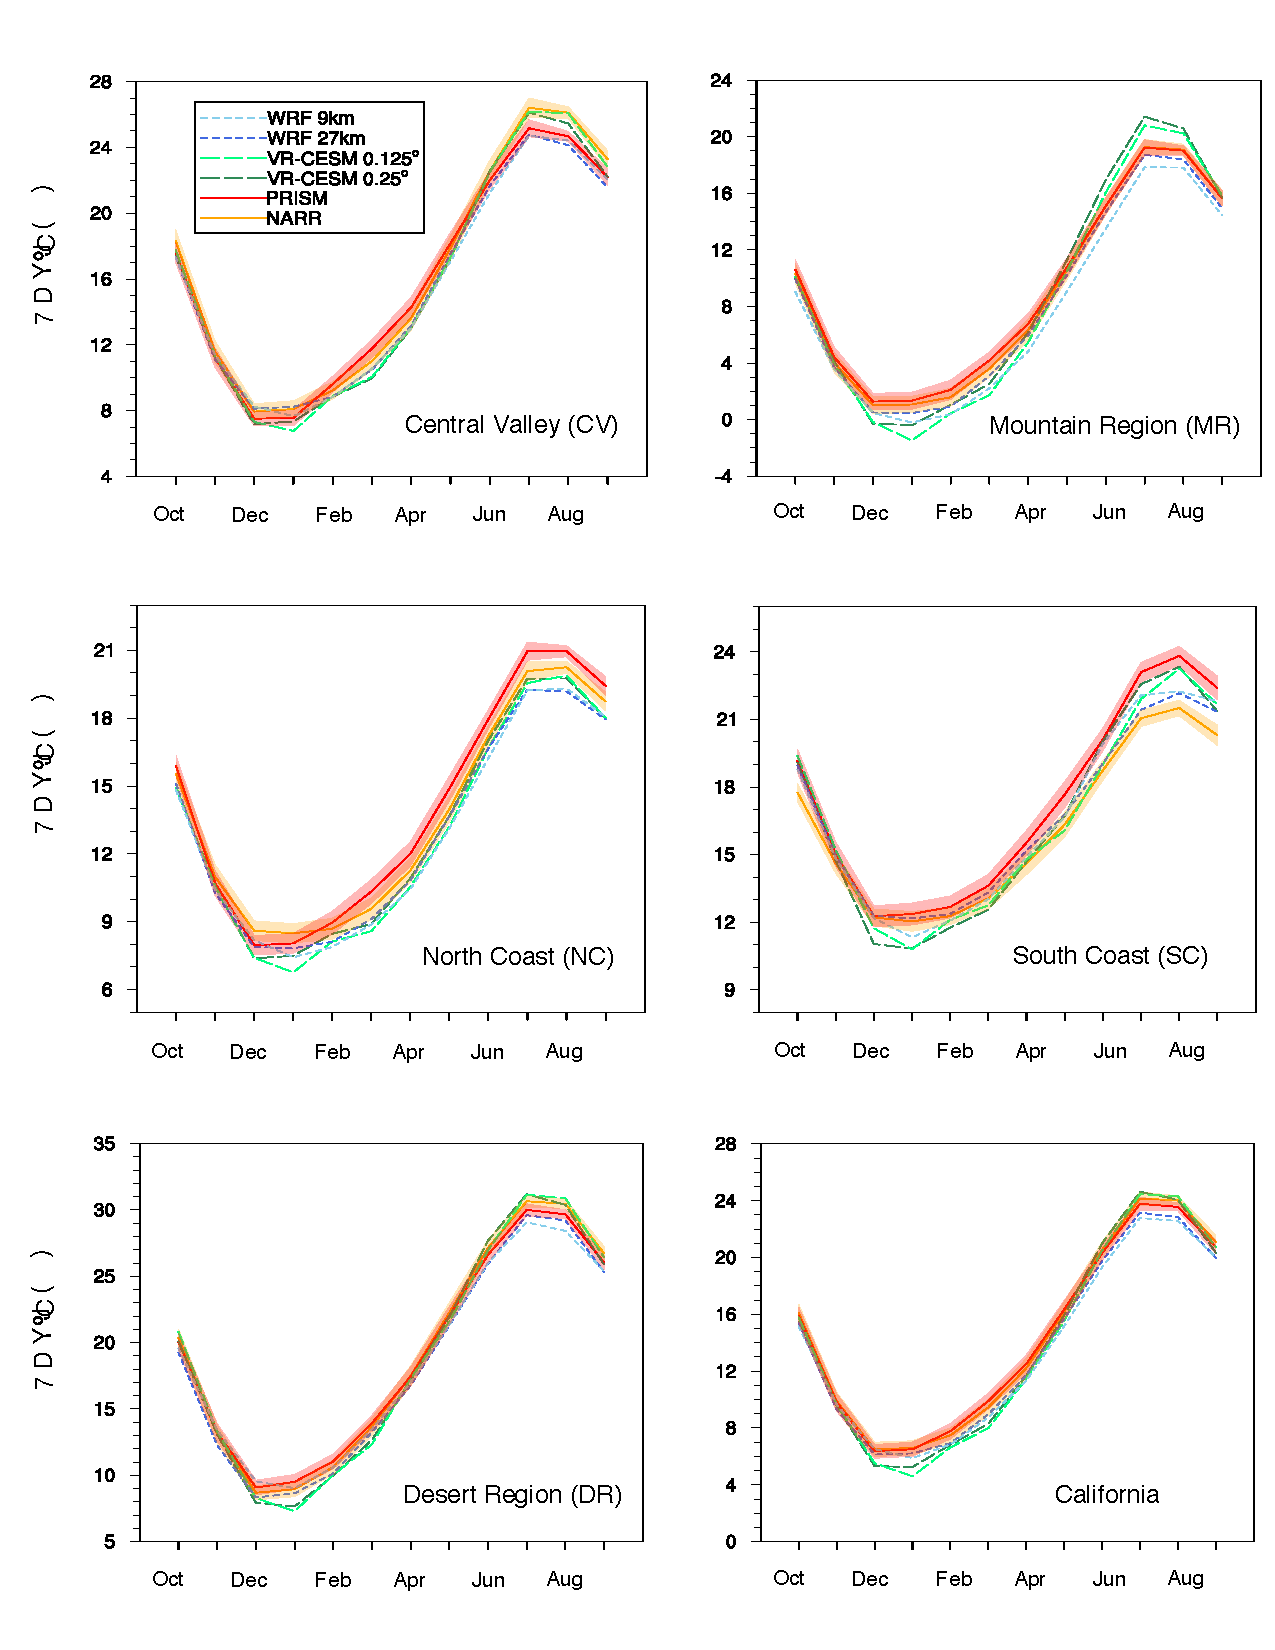
\includegraphics[width=6in]{trd_t2avg_allzones.pdf}
\end{center}
\caption{Seasonal cycle of monthly-average Tavg for each subzone ($^\circ C$). Bars represent standard deviation ($\sigma$) values.} \label{fig:trd_t2avg_allzones}
\end{figure}

\begin{figure}
\begin{center}
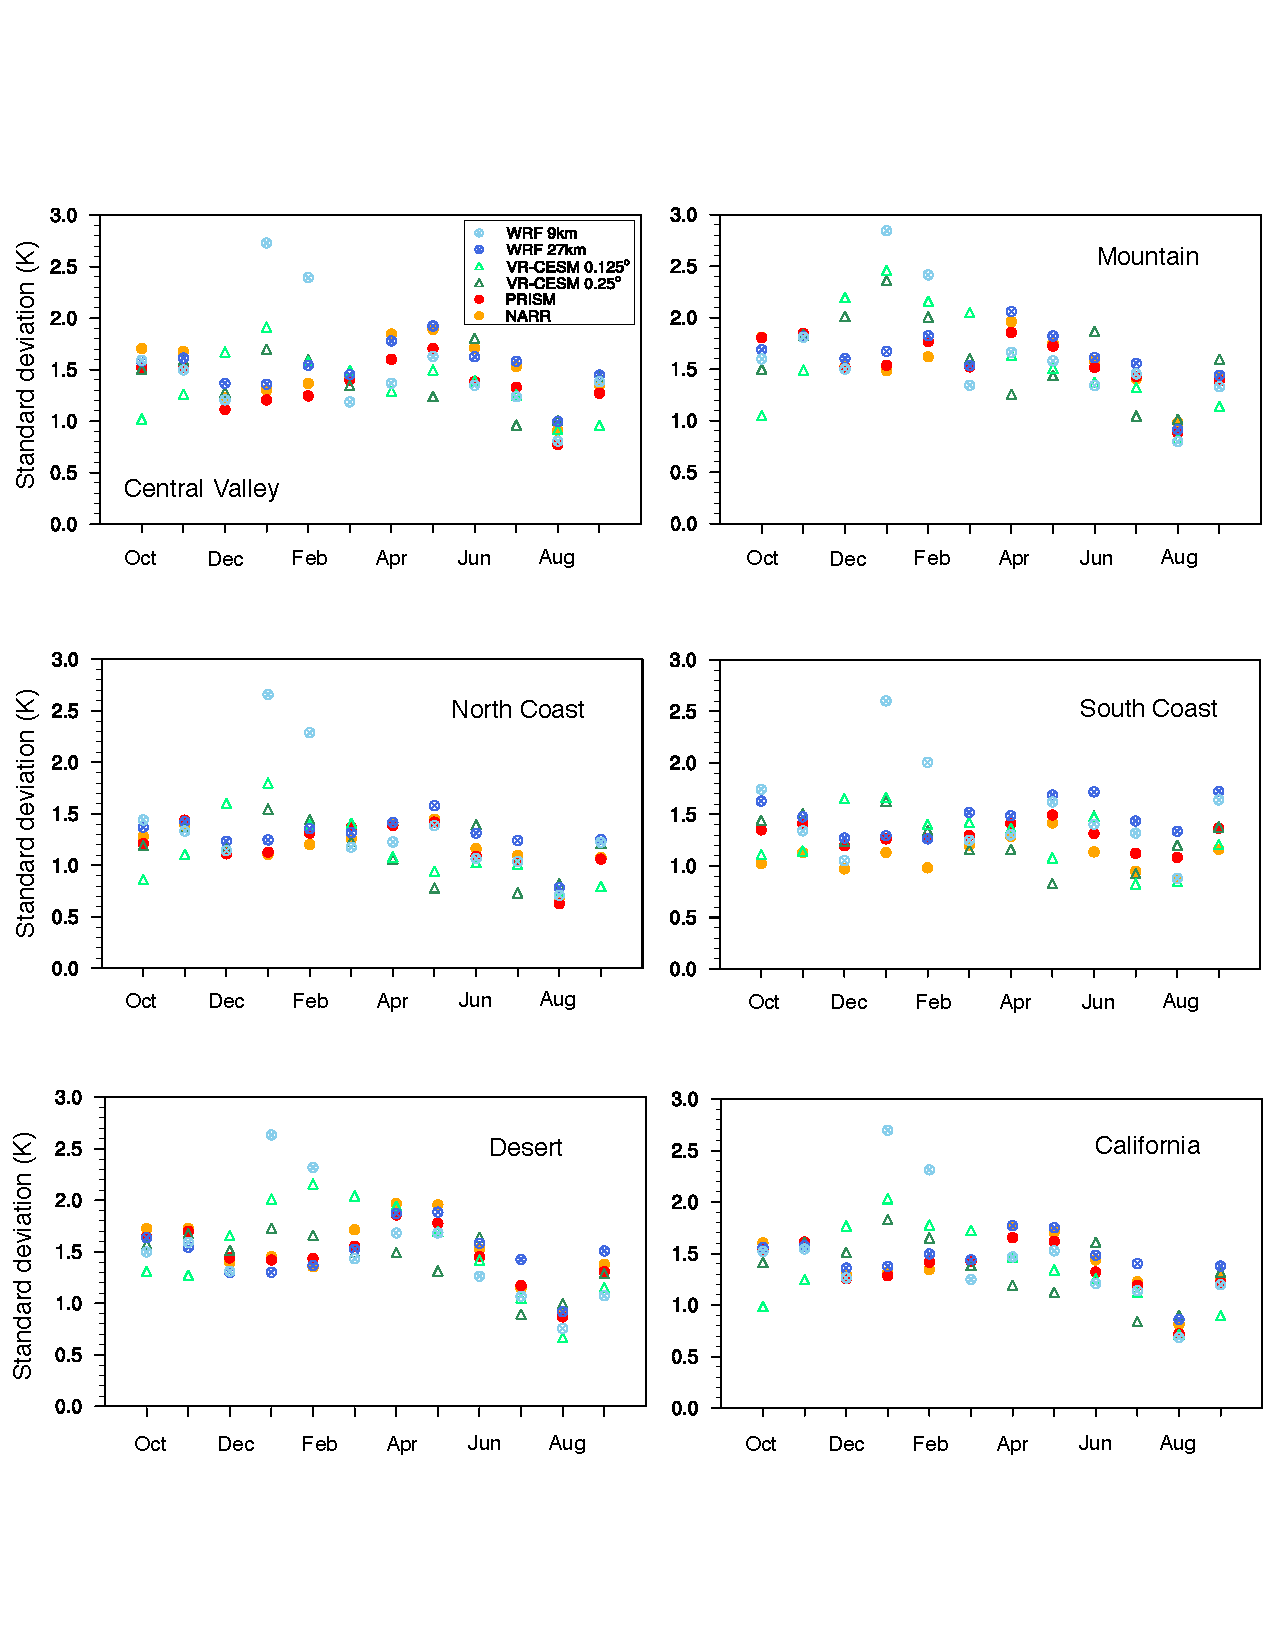
\includegraphics[width=6in]{trd_t2avg_allzones_std.pdf}
\end{center}
\caption{Seasonal standard deviation ($s$) values of monthly-average Tavg for each subzone ($^\circ C$). Bars represent standard deviation ($s$) values.} \label{fig:trd_t2avg_allzones_std}
\end{figure}


\begin{figure}
\begin{center}
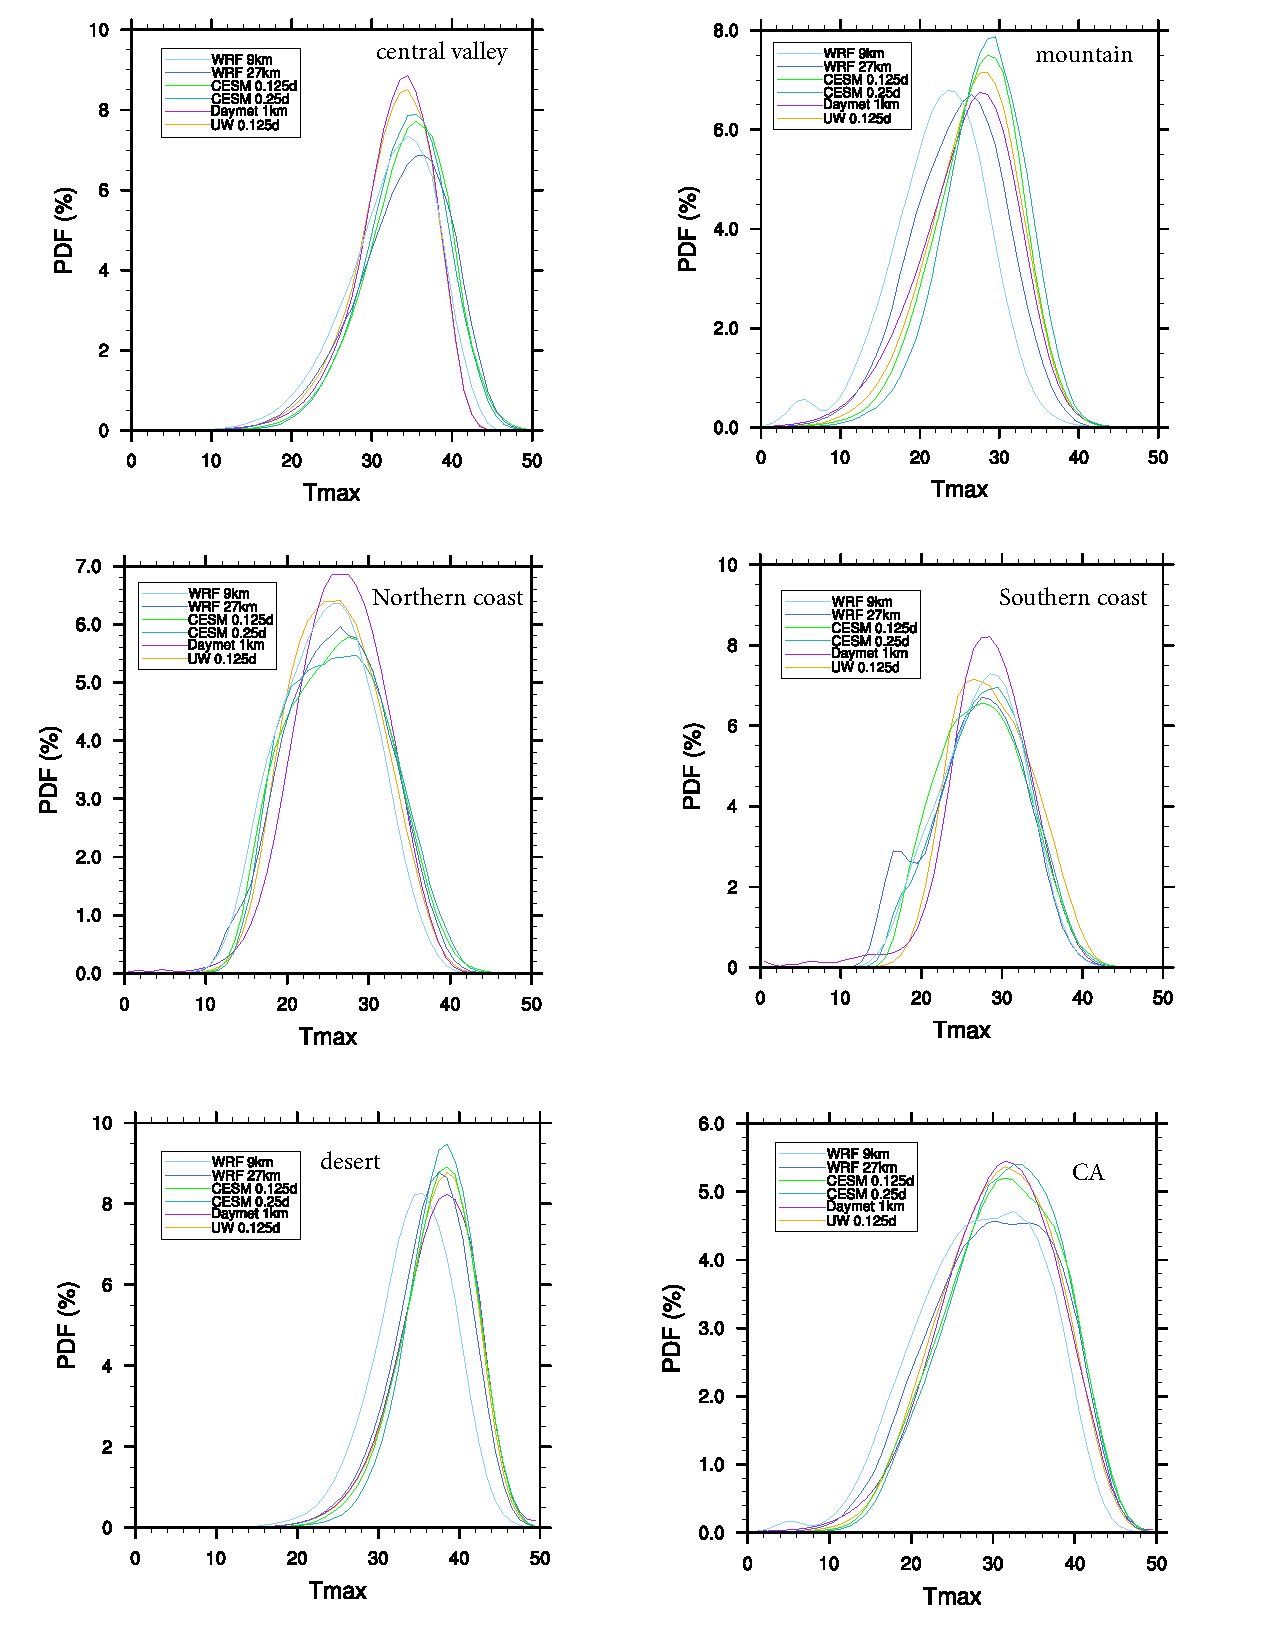
\includegraphics[width=6in]{PDF_t2max_allzones_JJA.pdf}
\end{center}
\caption{Frequency distribution of summer Tmax ($^\circ C$).} \label{fig:PDF_t2max_allzones_JJA}
\end{figure}


\begin{figure}
\begin{center}
\includegraphics[width=6in]{pr_DJF_Annual.pdf}
\end{center}
\caption{Annual and DJF precipitation from models and reference datasets (mm/d).} \label{fig:pr_DJF_Anuual}
\end{figure}

\begin{figure}
\begin{center}
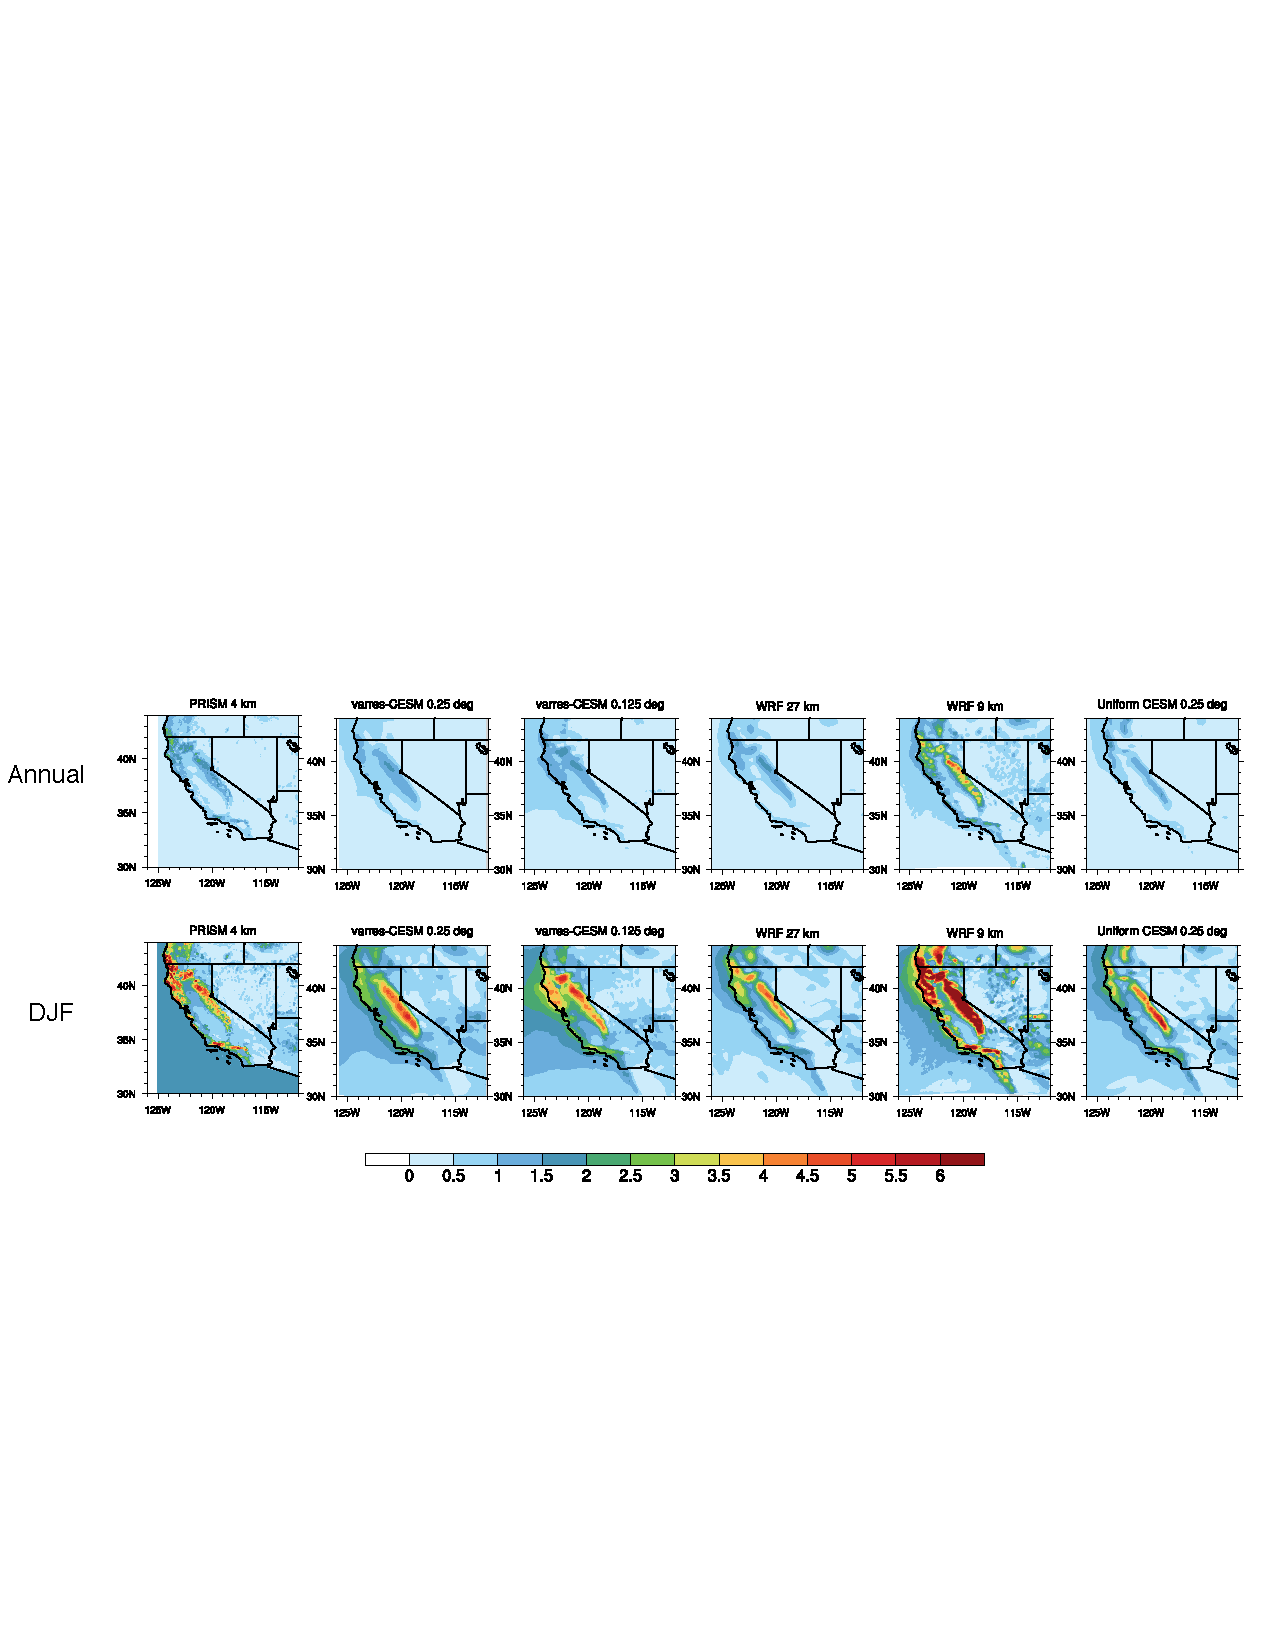
\includegraphics[width=6in]{pr_DJF_Annual_std.pdf}
\end{center}
\caption{sample standard deviation of Annual and DJF precipitation from models and PRISM (mm/d).} \label{fig:pr_DJF_Annual_std}
\end{figure}

\begin{figure}
\begin{center}
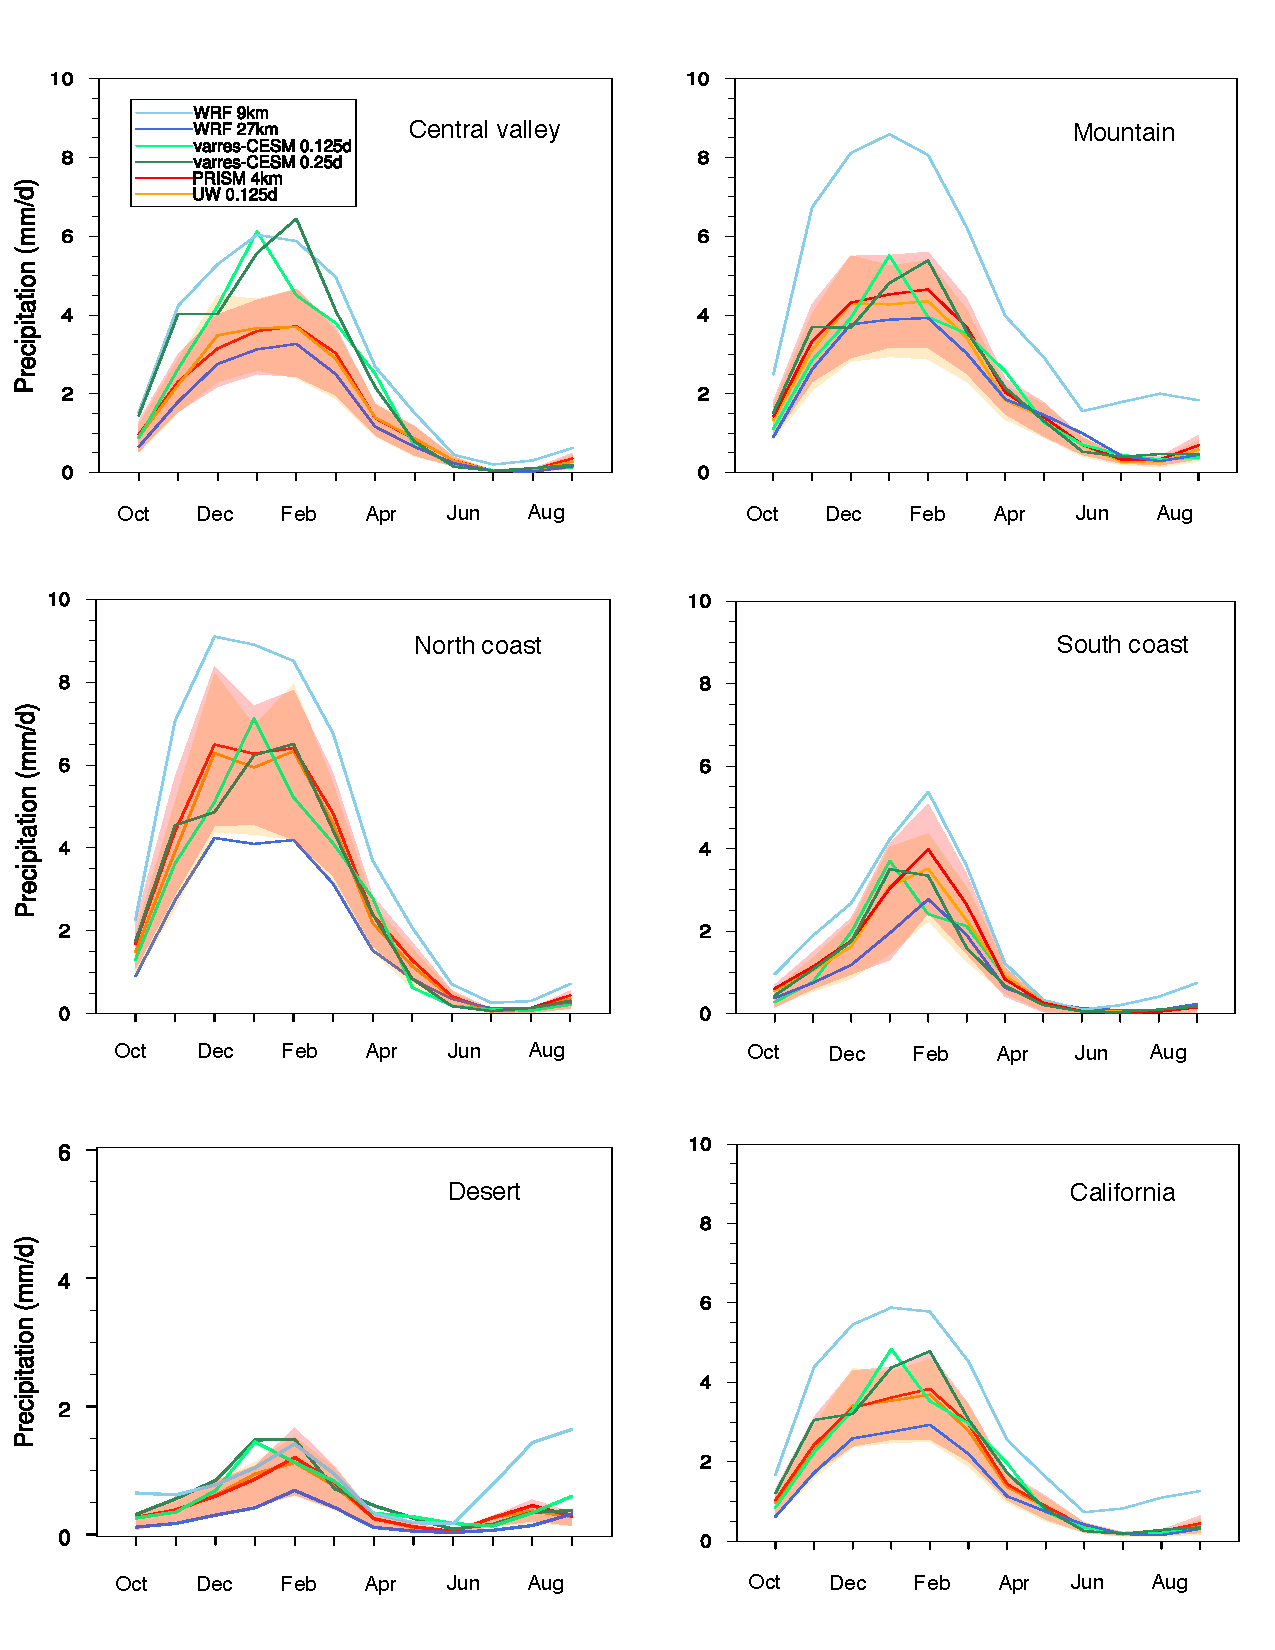
\includegraphics[width=6in]{trd_pr_allzones.pdf}
\end{center}
\caption{As Figure 6, but for monthly-average total precipitation (mm/d).} \label{fig:trd_pr_allzones}
\end{figure}

\begin{figure}
\begin{center}
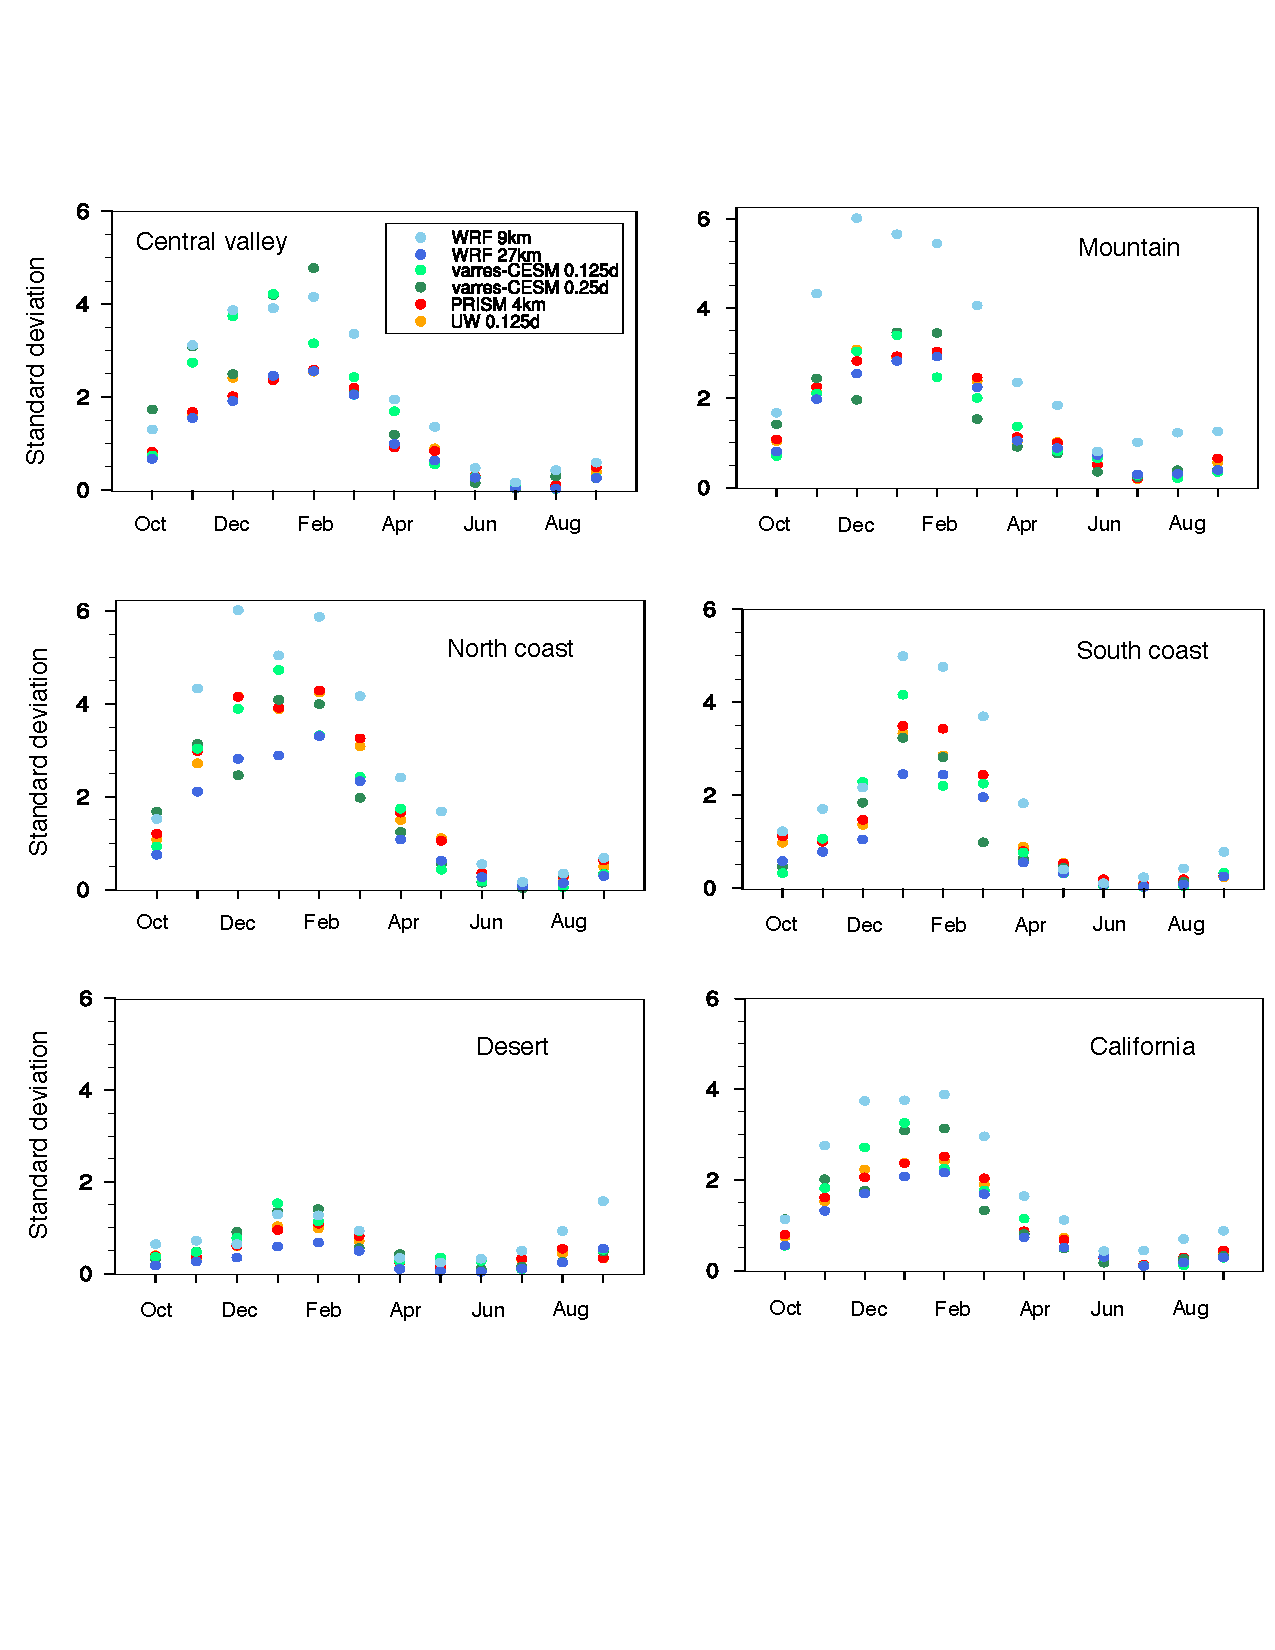
\includegraphics[width=6in]{trd_pr_allzones_std.pdf}
\end{center}
\caption{As Figure 7, but for monthly-average total precipitation (mm/d).} \label{fig:trd_pr_allzones_std}
\end{figure}

\begin{figure}
\begin{center}
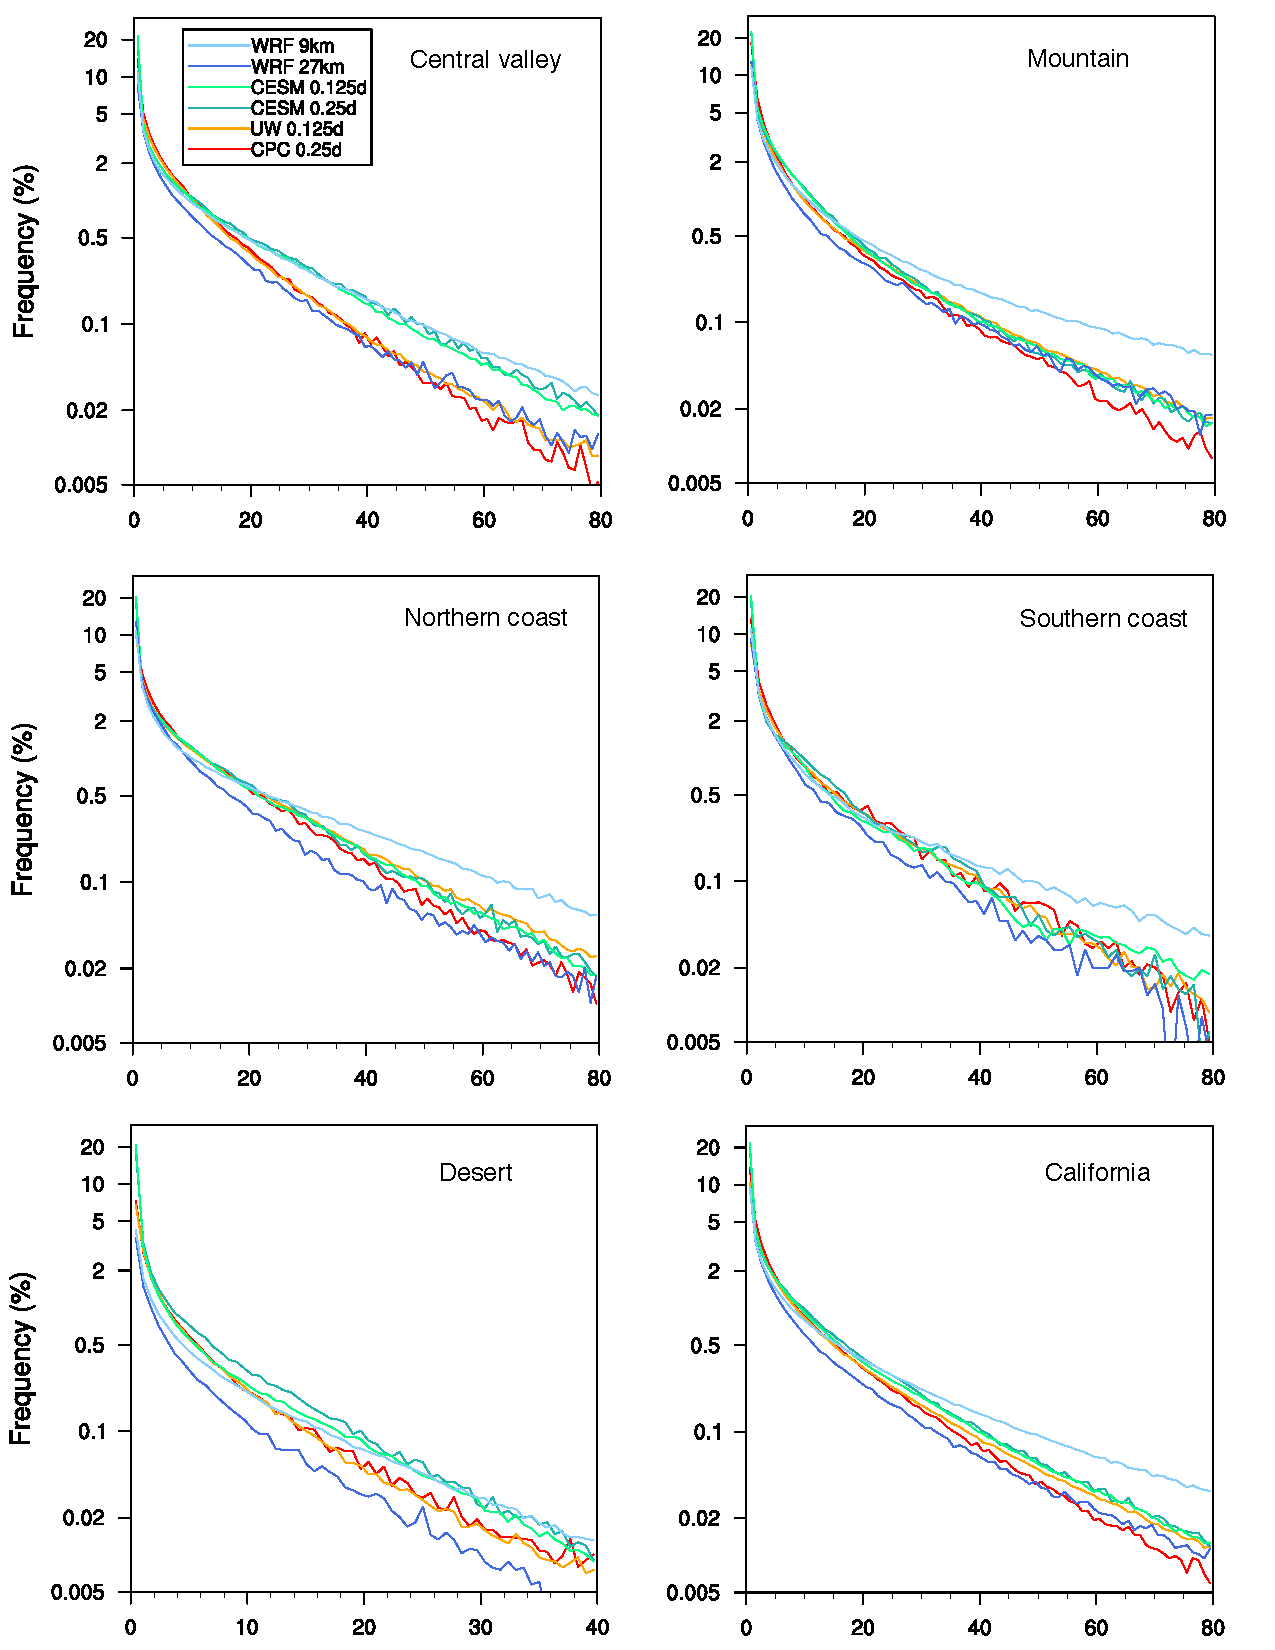
\includegraphics[width=6in]{PDF_pr_allzones_DJF.pdf}
\end{center}
\caption{Frequency distribution of winter Pr constructed from 26 years of daily data (mm/d) (note that the vertical scale is logarithmic).} \label{fig:PDF_pr_allzones_DJF}
\end{figure}

\begin{figure}
\begin{center}
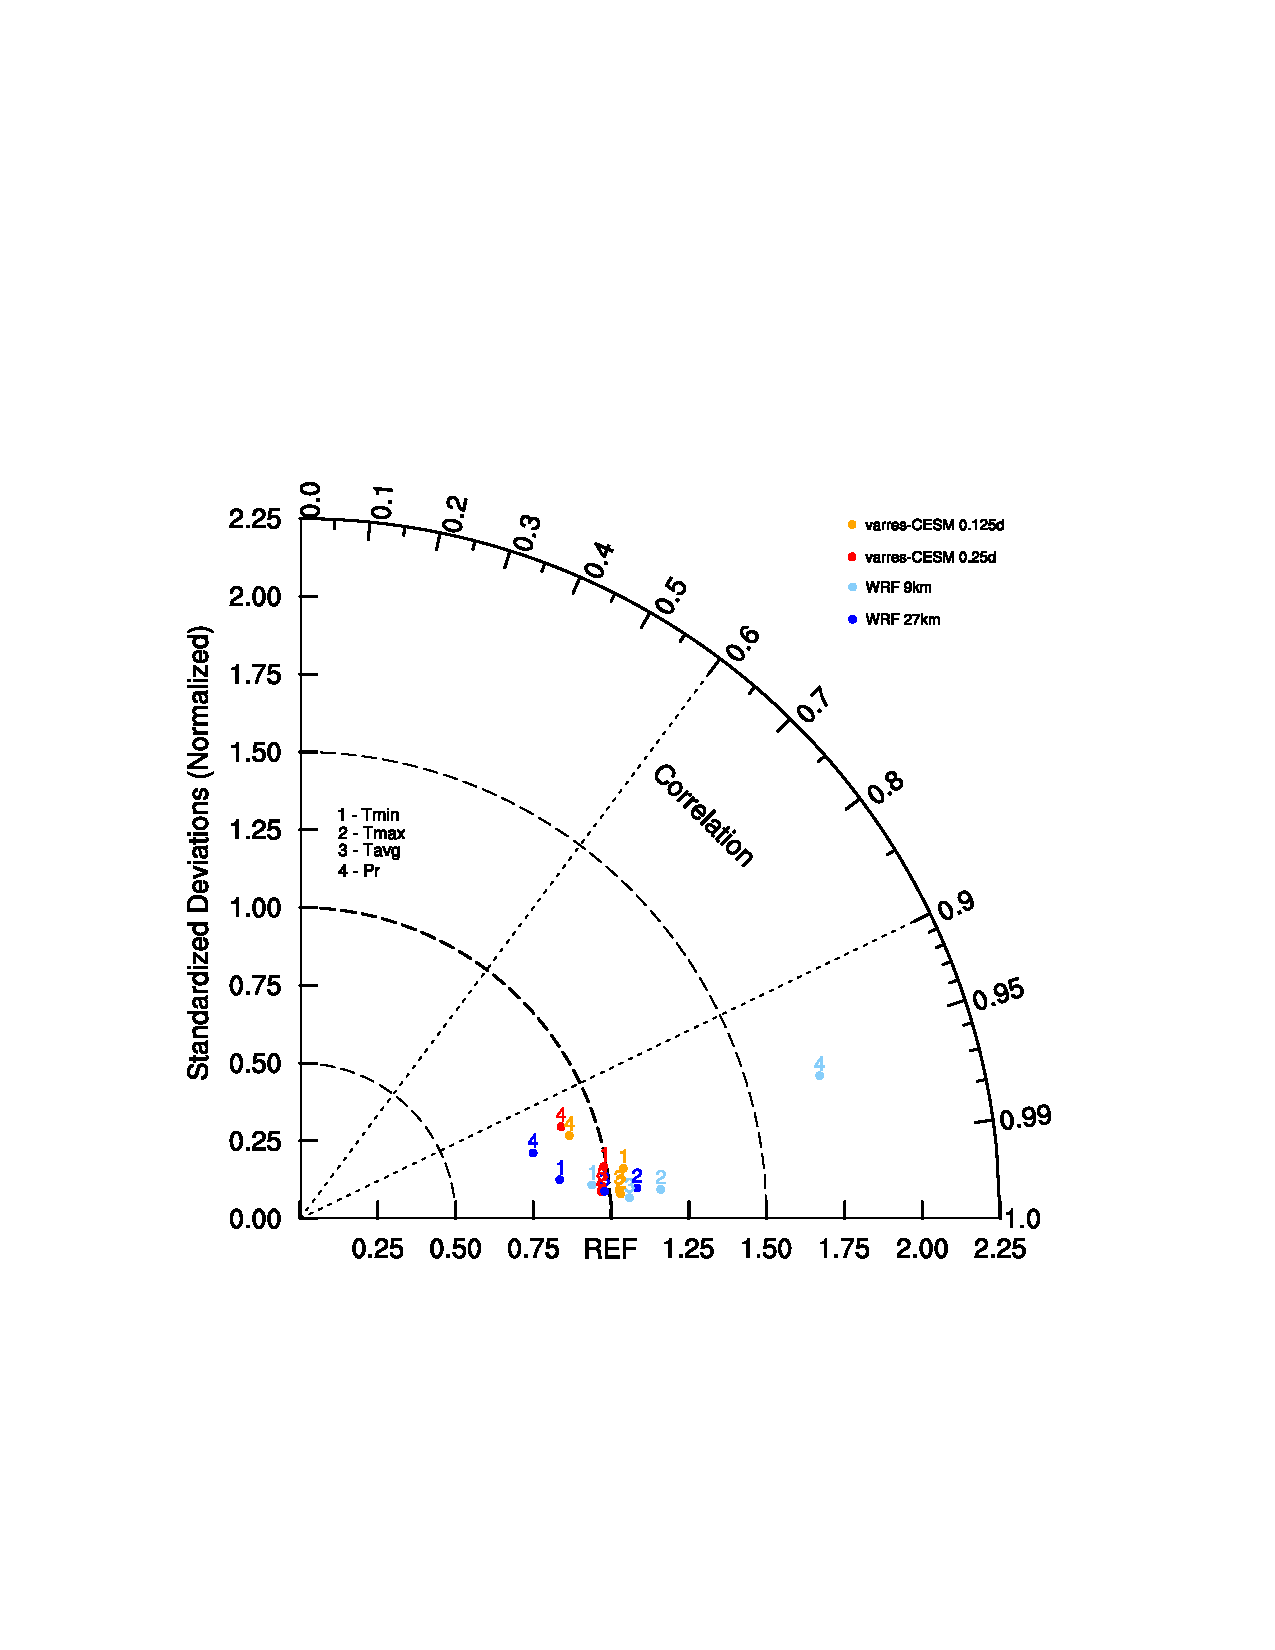
\includegraphics[width=6in]{taylor_diagram.pdf}
\end{center}
\caption{Taylor diagram of annual climatology for the entire California region, using the PRISM dataset as reference.} \label{fig:taylor_diagram}
\end{figure}

%upload grid, namelist file and settings files so that people can reproduce 
%probably at the last to come up a table that containing all the diagnostic variables and the corresponding model that works best. maybe not.


%%%%%%%%%%%%%%%%%%%%%%%%%%%%%%%%%%%%%%%%%%%%%%%%%%%%%%%%%%%%%%%%%%%%%
% END OF AMSPAPER.TEX
%%%%%%%%%%%%%%%%%%%%%%%%%%%%%%%%%%%%%%%%%%%%%%%%%%%%%%%%%%%%%%%%%%%%%

%%%%%%%%%%%%%%%%%%%%%

\end{document}
